% %
% LAYOUT_E.TEX - Short description of REFMAN.CLS
%                                       99-03-20
%
%  Updated for REFMAN.CLS (LaTeX2e)
%
\documentclass[a4paper]{refart}
\usepackage{makeidx}
\usepackage{ifthen}
\usepackage{graphicx}
\usepackage{amsmath}
\usepackage{amsfonts}
\usepackage{tabularx}
\usepackage{url}
\usepackage{hyperref}
\hypersetup{
    colorlinks=true,
    linkcolor=blue,
    filecolor=magenta,      
    urlcolor=blue,
    citecolor=blue
}
\usepackage{dirtree}
\usepackage[labelfont=bf]{caption}

\usepackage[backend=biber,style=numeric,
            sorting=none, natbib=true]{biblatex} % Complete re-implementation of bibliographic facilities
\addbibresource{references.bib}

\def\bs{\char'134 } % backslash in \tt font.
\newcommand{\ie}{i.\,e.,}
\newcommand{\eg}{e.\,g..}
\DeclareRobustCommand\cs[1]{\texttt{\char`\\#1}}

\title{Indoor Chemical Model (INCHEM-Py v1.1) \\
User Manual\\
\begin{figure}
    \hspace{-0.25\textwidth}\hspace{0.25in}
    
\includegraphics[width=\textwidth]{INCHEMPY_logo.png}
\end{figure}}

\author{
David Shaw\\
\texttt{david.shaw@york.ac.uk}\\
Nic Carslaw\\
\texttt{nicola.carslaw@york.ac.uk}\\
}

\date{Updated: \today}
\emergencystretch1em  %

\pagestyle{myfootings}
\markboth{INCHEM-Py}%
         {INCHEM-Py}

\makeindex 

\setcounter{tocdepth}{2}

\begin{document}

\maketitle


%\begin{abstract}
%abstract
%\end{abstract}
\newpage
\tableofcontents


\vspace*{\fill}

Copyright \textcopyright \hspace{1mm}2019-2021 \\
David Shaw : david.shaw@york.ac.uk\\
Nicola Carslaw : nicola.carslaw@york.ac.uk\\


Permission is granted to copy, distribute and/or modify this
document under the terms of the GNU Free Documentation License,
Version 1.3 or any later version published by the Free Software
Foundation; with no Invariant Sections, no Front-Cover Texts, and
no Back-Cover Texts.  A copy of the license is available at \url{https://www.gnu.org/licenses/fdl-1.3.html}.

%%%%%%%%%%%%%%%%%%%%%%%%%%%%%%%%%%%%%%%%%%%%%%%%%%%%%%%%%%%%%%%%%%%%

\newpage
\section{INCHEM-Py overview}
The INdoor CHEMical model in Python (INCHEM-Py) is an open source box model that creates and solves a system of coupled Ordinary Differential Equations (ODEs) to provide predicted concentrations of indoor air pollutants through time. It is a refactor of the indoor detailed chemical model, developed by Carslaw  \cite{Carslaw2007}, with improvements in form, function, and accessibility.

INCHEM-Py uses the Master Chemical Mechanism (MCM) \cite{Jenkin1997,Saunders2003,Bloss2005,Jenkin2012,Jenkin2015}, a near explicit mechanism developed for atmospheric chemistry, with additional chemical mechanisms developed specifically for indoor air. These include gas-to-particle partitioning for three of the commonly encountered terpenes indoors (limonene and alpha- and beta-pinene), improved photolysis parameterisation, indoor-outdoor air exchange, and deposition to surfaces. 

Typical usage of INCHEM-Py is either alongside experiment, where it can be used to gain a deeper insight into the chemistry through its ability to track a vast array of species concentrations; or as a standalone method of investigating chemical events that occur indoors over a range of conditions. INCHEM-Py is open source, has no black box processes, and all inputs can be tracked through the model allowing for complete understanding of the system.  

A wide array of outputs from the model can be accessed, including species concentrations, species reactivity and production rates, photolysis values, and summations such as the total peroxy radical concentration. Custom reactions and summations can also be added by users to tailor the model to specific indoor scenarios.

INCHEM-Py will continue to be developed into the future and new versions will be publicly released alongside peer reviewed literature. 

\section{Quick Start Guide}\index{Quick start}\label{Quick start}
\vspace{0.2cm}
{\hspace*{-\leftmarginwidth}
\begin{minipage}{\fullwidth}
If you're new to Python then the following guide will take you through a quick way to download the model, run the model and access the outputs.
\linespread{2.0}\selectfont
\begin{enumerate}
    \item Download Anaconda 3 from \url{https://www.anaconda.com/products/individual}
    \item Install Anaconda 3 with default settings. This is both your Python install and all of the required packages.
    \item Download INCHEM-Py from \url{https://github.com/DrDaveShaw/INCHEM-Py}
    \item Extract INCHEM-Py to the folder you would like to run it from
    \item Open Anaconda Navigator and "Launch" Spyder. If the "Launch" button says "Install" then you need to install it first.
            
            \vspace{1em}
            \begin{minipage}[t]{\linewidth}
                \centering
                
\includegraphics[width = 0.4\textwidth]{Spyder.png}
            \end{minipage}
            
    \item Spyder can be used to run INCHEM-Py. First navigate to the folder where INCHEM-Py was extracted by clicking the folder icon in the top right of Spyder. Browse to the INCHEM-Py directory. Select the INCHEM-Py folder.
                
            \vspace{1em}
            \begin{minipage}[t]{\linewidth}
                \centering
                
\includegraphics[width = 1.5cm]{folder.png}
            \end{minipage}
          
    \item At the bottom of the top right window in Spyder, click the "files" tab. This will show the contents of the INCHEM-Py folder in this window.
                
            \vspace{1em}
            \begin{minipage}[t]{\linewidth}
                \centering
                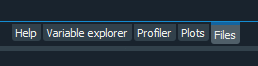
\includegraphics[width = 5cm]{files.png}
            \end{minipage}
          
\end{enumerate}
\end{minipage}}

\newpage
{\hspace*{-\leftmarginwidth}
\begin{minipage}{\fullwidth}
\linespread{2.0}\selectfont
\begin{enumerate}
\setcounter{enumi}{7}
    \item Double click on "settings.py" to open this file in the window on the left.
    \item To run INCHEM-Py click the green arrow in the Spyder tool bar.
                
            \vspace{1em}
            \begin{minipage}[t]{\linewidth}
                \centering
                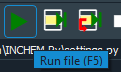
\includegraphics[width = 3cm]{run.png}
            \end{minipage}
          
          Progress will be shown in the console in the bottom right. It is normal for the first iteration to take a long time.
          
            \vspace{1em}
            \begin{minipage}[t]{\linewidth}
                \centering
                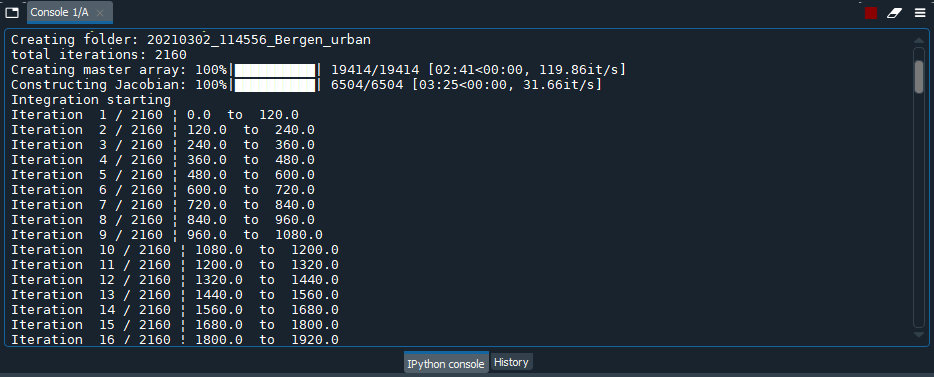
\includegraphics[width = 0.9\textwidth]{progress.png}
            \end{minipage}
            
          The output folder will also have been created in the INCHEM-Py directory with the current date and time, shown in the top right window. With default settings the model will take around 30~mins.
          
          The default plot of O$_3$ (O3 in the model) and O$_{3,outdoors}$ (O3OUT in the model) can be seen in the plots tab of the top right window, it is also saved in the created output folder as "graph.png" with these concentrations saved in csv format as "output.csv".
                    
            \vspace{1em}
            \begin{minipage}[t]{\linewidth}
                \centering
                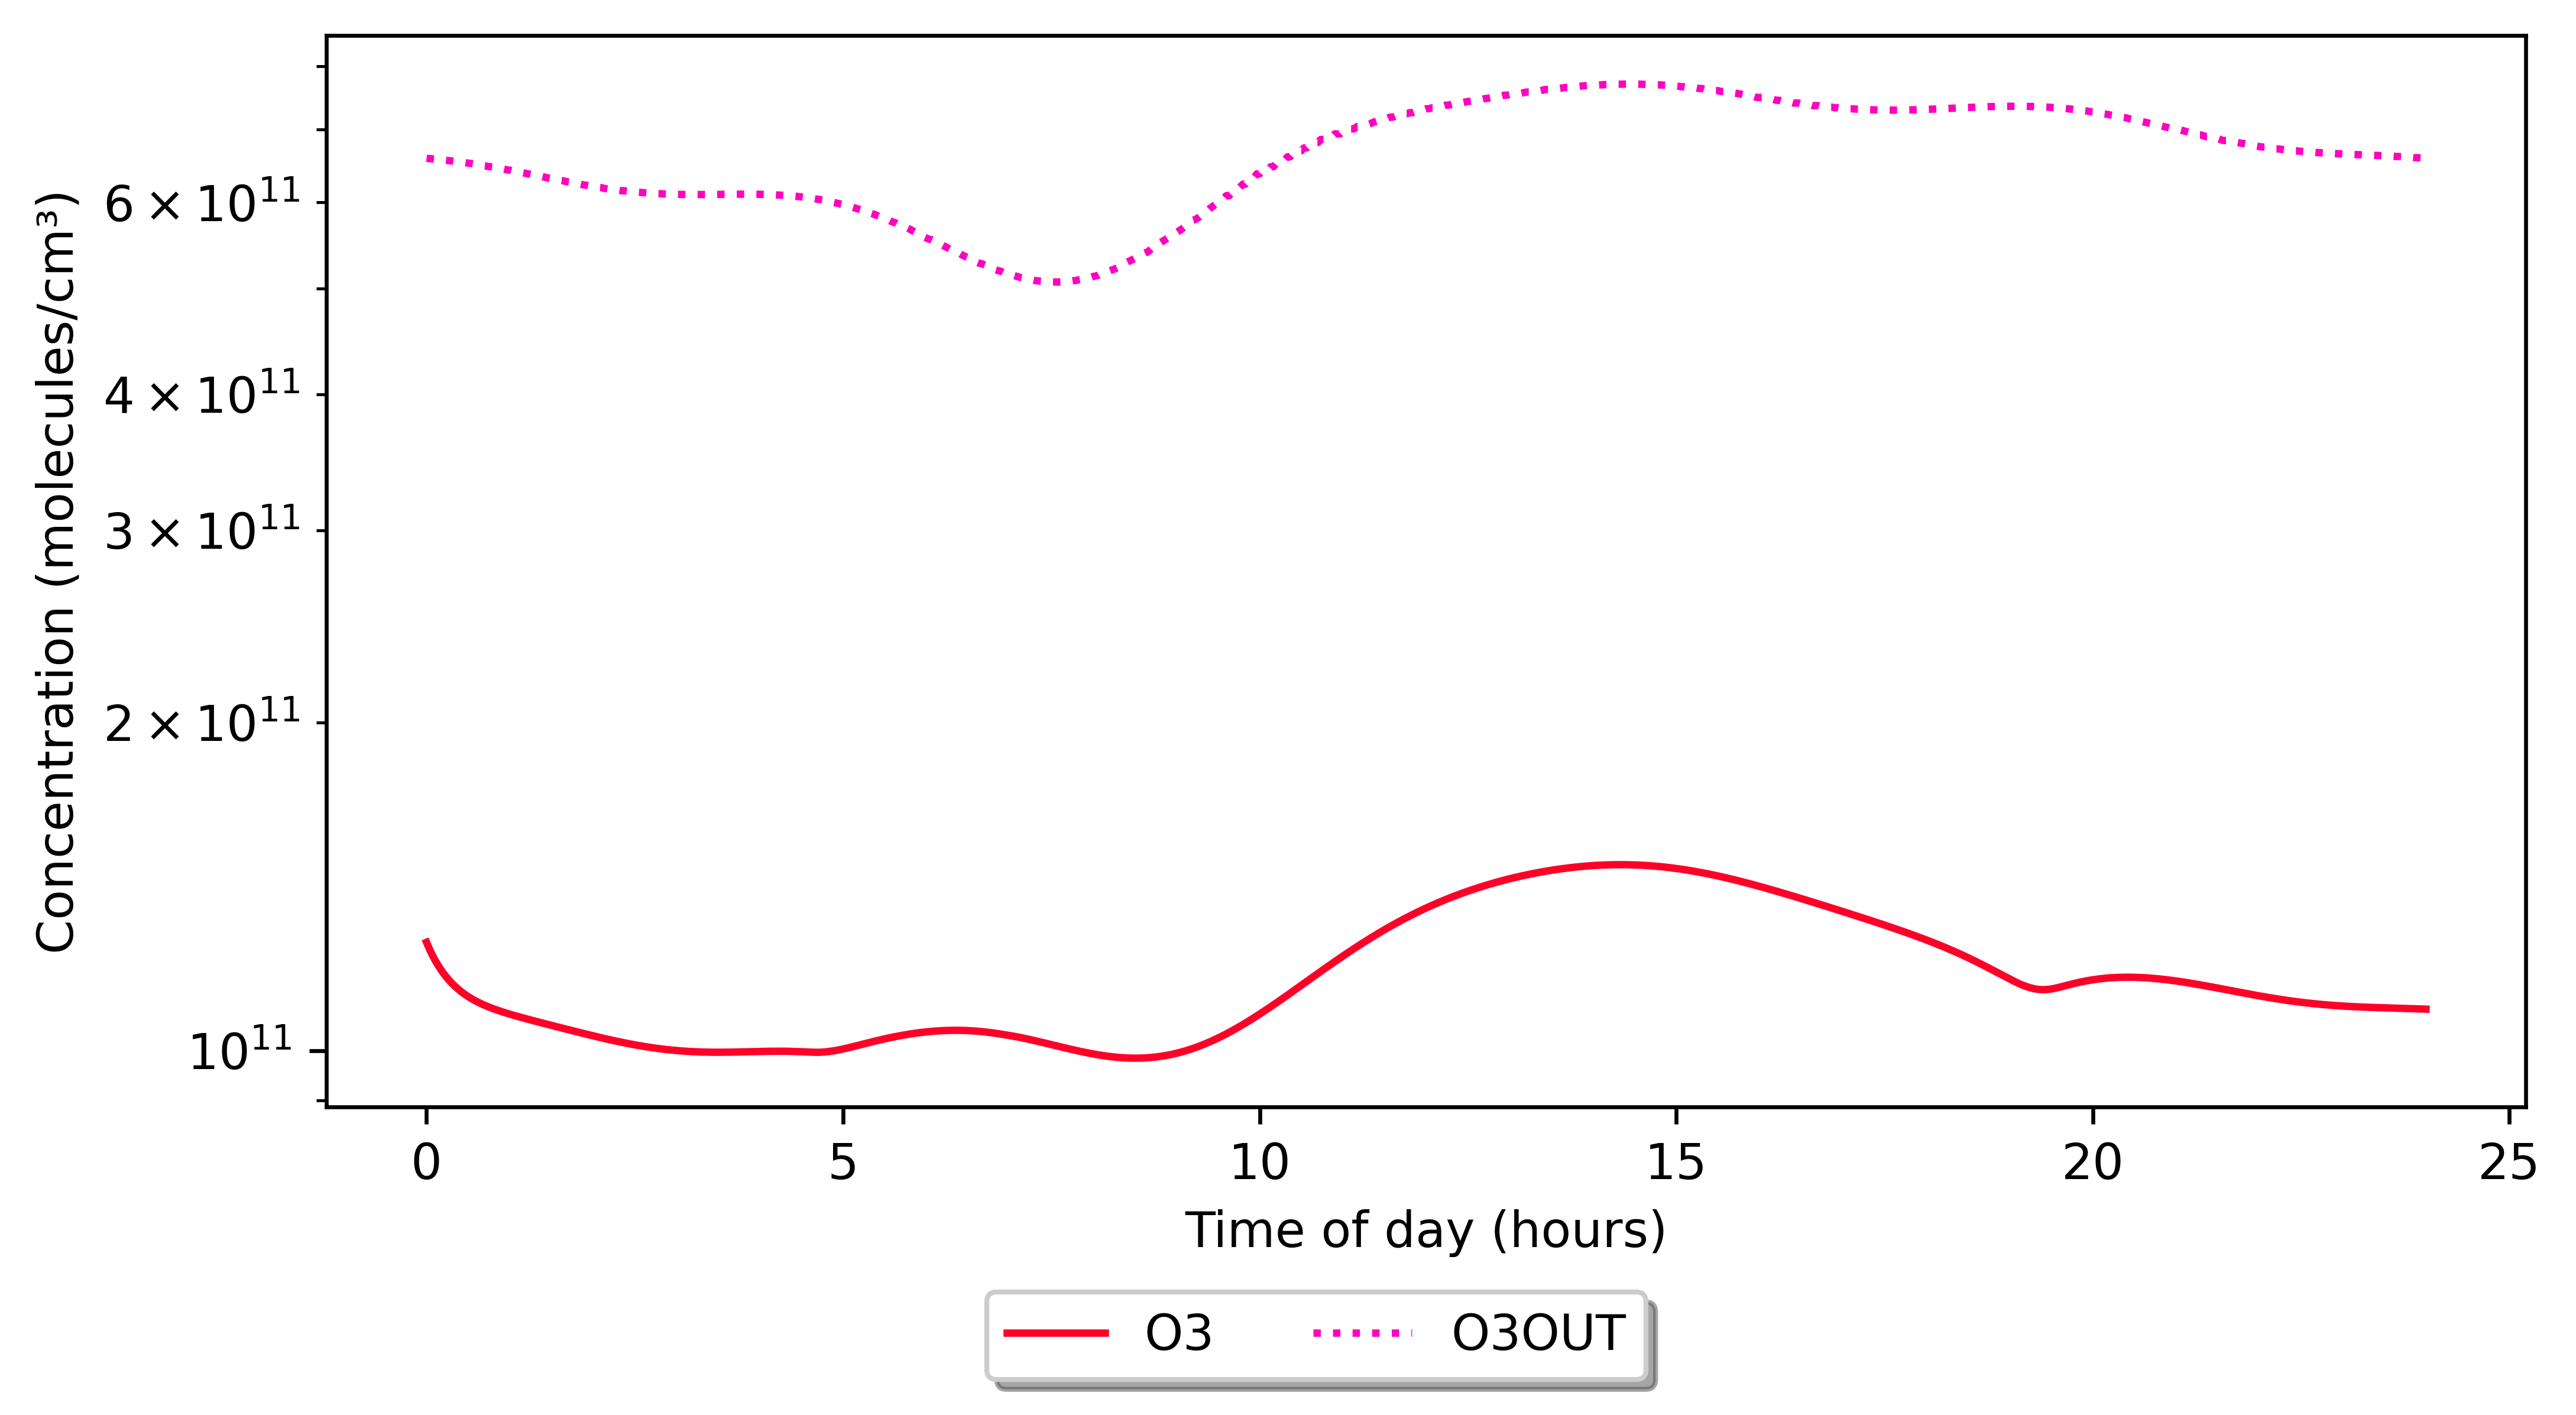
\includegraphics[width = 0.9\textwidth]{example_out.png}
            \end{minipage}

\end{enumerate}
\end{minipage}}

\newpage
{\hspace*{-\leftmarginwidth}
\begin{minipage}{\fullwidth}
\linespread{2.0}\selectfont
\begin{enumerate}
\setcounter{enumi}{9}
    \item The full output is saved in "out\_data.pickle". To extract other species concentrations to a csv file for analysis in other software the "inchem\_extractor.py" file is used. Double click on this file to open it in the left hand window. 
    
    The following variables can be changed to extract different outputs. Full details of these variables and how to change them can be found in appendix \ref{inchem_extractor.py}.
                        
            \vspace{1em}
            \begin{minipage}[t]{\linewidth}
                \centering
                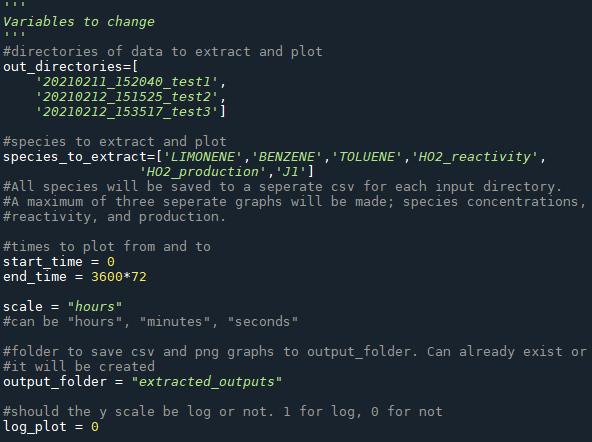
\includegraphics[width = 0.7\textwidth]{extractor.png}
            \end{minipage}

    \item To extract data from the model run that has just completed the "out\_directories" variable must be changed. The output folder in this example is "20210302\_114556\_Bergen\_urban" but will be slightly different for you. This name should be put into the "output\_directories" variable. 
                        
            \vspace{1em}
            \begin{minipage}[t]{\linewidth}
                \centering
                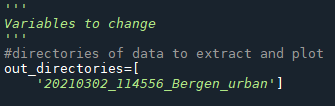
\includegraphics[width = 0.5\textwidth]{out_directories_variable.png}
            \end{minipage}
    
    \item To run the extractor, the same green arrow in the Spyder toolbar should be pressed.
                
            \vspace{1em}
            \begin{minipage}[t]{\linewidth}
                \centering
                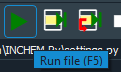
\includegraphics[width = 3cm]{run.png}
            \end{minipage}
          
          The folder "extracted\_outputs" is created and contains graphs for concentrations, reactivity, production rates, and photolysis of the default species in the extractor script. It also contains a csv file of all of these values from the simulation.
\end{enumerate}
\end{minipage}}

\newpage
\section{Dependencies}

\marginlabel{Installing Python}

INCHEM-Py relies on a number of Python packages. If you use Anaconda, then the current version at time of writing (Anaconda 2020.11) includes all of the packages required and no further downloads or installs are required.

If you have opted to not use Anaconda, are using an older version, or you have opened a new environment without the default packages, then the following packages need to be installed:
\begin{table}[h!]
    \centering
    \begin{tabular}{c|c}
        Package & Known working version \\
        \hline
        numpy & 1.19.2 \\
        numba & 0.51.2 \\
        pandas & 1.1.3 \\
        tqdm & 4.50.2 \\
        scipy & 1.5.2 \\
        threadpoolctl & 2.1.0 \\
        matplotlib & 3.3.2 \\
    \end{tabular}
\end{table}

\index{Downloading INCHEM-Py}\marginlabel{Downloading INCHEM-Py}

INCHEM-Py is available for download from \url{https://github.com/DrDaveShaw/INCHEM-Py} and should be extracted to the directory within the computer from which it will be run. This can be anywhere on the hard drive where there is sufficient space and where you have write permission. Each run of the model will save around 100 MB of data, depending on output options.


A version of the MCM is included in the INCHEM-Py download and is up-to-date as of February 2021, but should be updated if/when the MCM is updated.

\index{Downloading the MCM}\marginlabel{Downloading the MCM}\label{Downloading the MCM}

The Master Chemical Mechanism (MCM) can be downloaded from \href{http://mcm.leeds.ac.uk/MCM/}{the MCM website}.

INCHEM-Py has been designed to run with the full MCM mechanism.

In order to download a mechanism it first must be chosen via the \href{http://mcm.leeds.ac.uk/MCMv3.3.1/roots.htt}{"browse"} tab on the MCM website by checking the required subsets. "Check all" can be used to select everything, which INCHEM-Py has been designed to use. "Add Selection to Mark List" must then be used to add the checked subsets to your selection. Then the \href{http://mcm.leeds.ac.uk/MCMv3.3.1/extract.htt}{"extract"} tab can be used to download the mechanism or subset mechanism in the required format. This is the "FACSIMILE input format, suitable for inserting into a FACSIMILE model", also selecting the inclusion of inorganic reactions if required and the generic rate coefficients. Selecting "Extract" will download the required .fac file.

\newpage
\index{Folder structure}\marginlabel{Folder structure}

The following files show the folder structure of INCHEM-Py after extraction. If the model does not run, it could be due to missing files, please check that they are all downloaded and extracted correctly.
\dirtree{%
 .1 /. 
 .2 INCHEM-Py/.
 .3 manual source files/.
 .3 modules/.
 .4 test\_files/.
 .5 custom\_input\_test.txt.
 .5 in\_data.pickle. 
 .5 inchem\_test.py. 
 .5 initial\_test.txt.
 .5 jacobian\_test.txt.
 .5 mcm\_parse\_test.fac.
 .4 inchem\_import.py.
 .4 inchem\_main.py.
 .4 inchem\_test.py.
 .4 inchem\_chemistry.py.
 .4 initial\_dictionaries.py.
 .4 outdoor\_concentrations.py.
 .4 particle\_input.py.
 .4 photolysis.py.
 .4 reactivity.py.
 .4 surface\_dictionary.py.
 .3 custom\_input.txt.
 .3 inchem\_extractor.py.
 .3 INCHEMPY\_logo.png.
 .3 INCHEMPY\_logo.svg.
 .3 initial\_concentrations.txt.
 .3 LICENSE.
 .3 mcm\_v331.fac.
 .3 README.md.
 .3 settings.py.
 }

\newpage
\section{Model set-up}
INCHEM-Py consists of a number of input files and a single settings file in which the model options can be specified. The files themselves are all commented, but a description is also provided below.

\subsection{Naming conventions}\index{Naming conventions}\label{Naming conventions}
All species names are in the format given by the MCM download. There is no guide to these but they are self explanatory in most cases. If you are unsure of a species name, then check using \href{http://mcm.leeds.ac.uk/MCM/}{the MCM website} and search for the species using its MCM name or SMILES string.

When using custom inputs it is important that any new species do not share a name with any of the existing species, including those used in the inchem\_chemistry file inputs.\seealso{\hyperref[custom_input.txt]{custom\_input.txt}}

Other names are assigned within INCHEM-Py. \seealso{\hyperref[outputs]{outputs}}The following naming conventions are used:
\begin{itemize}
    \item \texttt{J1, J2, J3, etc...} - photolysis rates, combining indoor artificial lighting and attenuated sunlight according to the selected conditions \seealso{\hyperref[photolysis.py]{photolysis}}
    \item \texttt{O3OUT, HONOOUT, NOOUT, etc...} - outdoor concentrations. Not all species have outdoor concentrations and the majority are constants. The specified outdoor concentrations are listed in the outdoor\_concentrations.py module
    \item \texttt{tsp} - total suspended particles (molecules cm$^{-3}$) and \texttt{tspx} - total suspended particles in $\mu$g/m$^3$, PM 2.5, if particles are used \seealso{\hyperref[particles]{particles}}
    \item \texttt{OH\_reactivity, OH\_production, etc...} - the reactivity and production rates of species specified in the reactivity.py module \seealso{\hyperref[reactivity.py]{reactivity and production}}
    \item \texttt{RO2} - the sum of all organic peroxy radical concentrations
\end{itemize}

\subsection{settings.py}\label{settings.py}
The settings file provides inputs for all of the current model variables and runs the model. All species names must be in the MCM format. The following variables are used in the model and can be adjusted. Each must have a value even if unused.

\index{filename}\marginlabel{filename}
\texttt{"mcm.fac"}\\ 
The file name for the download of the MCM from the MCM website. The format and placement of the file within the file structure is detailed earlier in this document. \seealso{\hyperref[Downloading the MCM]{Downloading the MCM}}

\index{particles}\marginlabel{particles}
\label{particles}
\texttt{True or False}\\
Set to True to include gas-to-particle partitioning for limonene, alpha-pinene and beta-pinene within the simulation and to False to exclude particle formation. Details of how particles are implemented can be found in Carslaw et al. (2012), which is based on the methodology of Pankow (1994) \cite{Carslaw2012,Pankow1994}.

\index{inchem\_chemistry}\marginlabel{inchem\_chemistry}
\texttt{True or False}\\
Set as True to use the inchem\_chemistry.py module which includes additional reaction mechanisms developed specifically for indoor air chemistry. \seealso{\hyperref[inchem_chemistry]{INCHEM reactions}}

\index{custom}\marginlabel{custom}
\texttt{True or False}\\
Set as True to use the custom\_input.txt file to include user set reactions that are not included in the MCM. Set as False to ignore custom\_input.txt. The formatting of this file is detailed within the file itself and also within the \seealso{\hyperref[custom_input.txt]{custom\_input.txt}} custom\_input.txt section of this document.

\index{temp}\marginlabel{temp}
\texttt{293 K}\\
Temperature in degrees Kelvin. Set to 293 K as default value.

\index{rel\_humidity}\marginlabel{rel\_humidity}
\texttt{50 \%}\\
Relative humidity as a percentage. Set to 50\% as default value.

\index{M}\marginlabel{M}
\texttt{2.51e+19}\\
Number density of air in the simulated environment in molecules cm$^{-3}$.

\index{const\_dict}\marginlabel{const\_dict}
\texttt{\{'species' : number density in molecules cm$^{-3}$\}}\\
Dictionary of species or values that should remain constant throughout the simulation. There is no limit to the number of species that can be included in this way and the code will remove them from the integration. O$_2$ and N$_2$ should always be included as the MCM does not include them as outputs in reactions due to their abundance in the atmosphere.

\index{AER}\marginlabel{AER}\label{AER}
\texttt{0.5/3600}\\
The Air Exchange Rate per second. The number of times the volume of air in the room is fully exchanged with the air from outside. In this example we want 0.5 changes per hour which is divided by 3600 to convert to per second. For reference, 0.2 is considered to be a reasonable value for a very well insulated building, 2.0 would be considered reasonable for a very loosely built building \cite{Weschler2000}.

\index{diurnal}\marginlabel{diurnal}
\texttt{True or False}\\
Set as True to include diurnal outdoor concentrations and as False to use constant values. These outdoor concentrations are for OH and HO2 radicals, NO, NO$_2$, tsp, O$_3$ and HONO. Both the diurnal equations and the constant values can be adjusted in the outdoor\_concentrations.py \seealso{\hyperref[outdoor_concentrations.py]{outdoor\_concentrations.py}} file within the modules folder.

\index{city}\marginlabel{city}
\texttt{"London\_urban", "London\_suburban", "Bergen\_urban",\\ or "Milan\_urban\_Aug2003"}\\
The model comes with four preset outdoor fits to measured concentrations for O$_3$, NO$_2$, NO, and PM 2.5. Three of these are daily average fits over the three month period of July - September for urban London, suburban London, and urban Bergen, respectively, in 2018. The Milan concentrations are fits taken from a particularly polluted two week period in Milan in August 2003 taken from Terry et al. (2014) \cite{Terry2014}. The full details of the locations and data can be found in the outdoor concentrations section of this manual. \seealso{\hyperref[outdoor_concentrations.py]{outdoor\_concentrations.py}} Although we do provide this data for use in the model it is clear that the outdoor concentrations can have a major effect on indoor air chemistry, therefore, we advise that tailored outdoor fits are produced for any specific location.

\index{date}\marginlabel{date}
\texttt{"10-11-2020"}\\
The day of the simulation in the format "DD-MM-YYYY" as a string. The model will use this date for all days simulated and is used for the photolysis calculations to work out the angle of the Sun.

\index{lat}\marginlabel{lat}
\texttt{45.4}\\
The latitude of the simulation location.

\index{light\_type}\marginlabel{light\_type}
\texttt{"Incand", "Halogen", "LED", "CFL", "UFT", "CFT", "FT", or "off"}\\
The type of indoor lighting used within the simulation as a string. Incand for incandescent, Halogen for halogen, LED for light emitting diodes, CFL for compact fluorescent lighting, UFT for uncovered fluorescent tubes, CFT for covered fluorescent tubes, and FT for fluorescent tubes. The values used for these are included in the photolysis.py \seealso{\hyperref[photolysis.py]{photolysis.py}} module and are taken from work done by Wang and Carslaw (2021) \cite{Wang2021}. "off" sets the attenuation factors of indoor lights to 0 and therefore removes indoor lighting from the simulation.

\index{light\_on\_times}\marginlabel{light\_on\_times}
\texttt{[[light on time (h), light off time (h)],[light on time (h), light off time (h)]]}\\
A list of times at which the indoor lights are turned on and turned off. These times are in hours from 00:00 on the first day of the simulation. E.g. an input of 7 would be 7 AM on the first day and an input of 31 would be 7 AM on the second day. These are irrespective of the time at which the simulation starts, if the simulation is set to start at 8 am and the lights are set to come on at 7 AM, then the simulation would start with the lights on. Decimals can be used to fine tune the times, e.g. 7.5 as an input would equate to 7:30 AM on the first day.

\index{glass}\marginlabel{glass}
\texttt{"glass\_C", "low\_emissivity", "low\_emissivity\_film", or "no\_sunlight"}\\
Type of window glass used for the attenuation of outdoor light by wavelength range as a string. The values are given in the photolysis.py module \seealso{\hyperref[photolysis.py]{photolysis.py}} and are based on the paper by Blocquet et al., (2018) \cite{Blocquet2018}. "no\_sunlight" sets all window attenuation factors to 0 and therefore no light enters from outdoors.

\index{HMIX}\marginlabel{HMIX}
\texttt{0.02}\\
Surface to volume ratio, used as a coefficient in the calculation of surface deposition. Individual species deposition rates can be adjusted in the surface\_dictionary.py \seealso{\hyperref[surface_dictionary.py]{surface\_dictionary.py}} file in the modules folder. Setting HMIX to 0 will remove surface deposition from the simulation.

\index{initials\_from\_run}\marginlabel{initials\_from\_run}\label{initials_from_run}
\texttt{True or False}\\
Initial gas concentrations are either provided by a text file (when initials\_from\_run = False and initial\_conditions\_gas is provided with the name of a text file) or by an output file from a previous run (when initials\_from\_run = True and providing an input as detailed below). 

The benefits of using an output file from a previous run are that the model will change the initial values depending on the start time of the simulation. E.g. if you set your model to run from 3600 seconds then by using initials\_from\_run the initial species concentrations will be from the 3600 second mark of the input file. The initial integration steps will be faster and require less time to equilibrate. This is especially useful if there is an event within the model, such as a timed input, which you are varying on multiple model runs and wish only to run the model over the short period where that event is occurring. 

To use data from a previous run for initialising species concentrations, the out\_data.pickle file from the run must be copied into the main folder of the model and renamed to in\_data.pickle with initials\_from\_run set to 1. The in\_data.pickle file must contain values for all species used in the current model run.

\index{initial\_conditions\_gas}\marginlabel{initial\_conditions\_gas}
\texttt{"initial.txt"}\\
The string file name of the text file containing the initial species concentrations in molecules cm$^{-3}$, the format of this file is detailed later in this document\seealso{\hyperref[initial_concentrations.txt]{initial\_concentrations.txt}}. If a species concentration is not given then the model will assume it is 0. To use this file, initials\_from\_run must be set to 0.

\index{timed\_emissions}\marginlabel{timed\_emissions}\label{timed emissions}
\texttt{True or False}\\
Set as False to not include additional emissions and True to include additional emissions. Emissions can be added at specific points in time during the simulation. The times and emission rates are set using timed\_inputs.

\index{timed\_inputs}\marginlabel{timed\_inputs}
\texttt{\{"species":[[start time, end time, rate]],\\
          "species2":[[start time, end time, rate],[start time, end time, rate]]\}}\\
A dictionary of species, times (s) and emissions rates  (molecules cm$^{-3}$ s$^{-1}$), for use when timed\_emissions is set to 1. The user needs to define the emission rates and times of emissions for their particular scenario in this file. In the above example, species2 emits at two different times at two different rates.

\seealso{\hyperref[timed emissions, implementation]{implementation of timed emissions}} As many species can be input this way as required. The model will still calculate changes in concentration over time during this input period. More details and examples are given later in this document.

\index{dt}\marginlabel{dt}
\texttt{120}\\
Time between outputs in seconds. \seealso{\hyperref[Integration]{Integration}}

\index{t0}\marginlabel{t0}
\texttt{0}\\
The time of day, in seconds from midnight, to start the integration. 

\index{seconds\_to\_integrate}\marginlabel{seconds\_to\_integrate}
\texttt{86400}\\
The length of the model run in seconds, starting at t=0. Arithmetic is accepted here so a simple way to run for four hours would be to input \texttt{3600*4}.

\index{custom\_name}\marginlabel{custom\_name}
\texttt{"string"}\\
String that is added to the end of the output folder name to make output folders easier to find and identify. 

\index{output\_graph}\marginlabel{output\_graph}
\texttt{True or False}\\
True to produce a graph of selected species (output\_species) and write it to file as "graph.png" in the output folder, False to not produce a graph. The species chosen will also have their concentrations saved in a csv format in the output folder in molecules cm$^{-3}$.

\index{output\_species}\marginlabel{output\_species}
\texttt{['species 1','species 2','species 3']}\\
A list of string names of species to be plotted on a graph if output\_graph is set to 1.

\subsection{custom\_input.txt (optional)}\label{custom_input.txt}
A file for inputting rates, reactions, additional peroxy radical species for the RO2 summation, as well as additional organic nitrate and PAN-type species for the summations of these that are not already included in the model. To use this file then custom in settings.py must be set to 1. This allows users to add custom mechanisms. A description of how to format the file is included here and within the file itself. Any species that are not already in the MCM download but that do appear in any of the additional custom equations will be automatically added to the species list. The user must be careful to spell the species names correctly. The user also needs to check that any new species formed on the right-hand side of a reaction, also appears on the left-hand side of at least one other reaction. Otherwise, the species would play no other part in the chemistry once formed. Finally, the user should be careful not to include species or reactions that are already in the model mechanism and should check against the species and reactions in the MCM and inchem\_chemistry.py carefully (it is possible to search the MCM by molecular weight and smiles string at \url{mcm.leeds.ac.uk}).

The format of any calculations (e.g. for rate coefficients) should be acceptable for Python, such as 'temp' for temperature. Any additional photolysis rates must be added in the appropriate module file and not here\seealso{\hyperref[photolysis.py]{photolysis.py}}.

\marginlabel{Rate Coefficients}
Rate coefficients in this file are common ones that might be used in multiple reactions within the file (e.g. KRO2NO for each time that a peroxy radical reacts with NO). These are simply entered as
\begin{verbatim}
    name = coefficient calculation
\end{verbatim}

\marginlabel{Reactions}
Reactions in this file are species reactions with their rate coefficients. The rate coefficients can include calculations, constants, common values included in the MCM (see previous section), additional values within this file, or a combination of these. The form that reactions should take is
\begin{verbatim}
    rate coefficient : species + species = species + species
    rate2 coefficient : species + species = species
\end{verbatim}
The code uses the colon and the mathematical symbols to parse the input so it is important that these are correct. There doesn't have to be a species on both sides of the reaction, pure loss or gain reactions are both valid, for example:
\begin{verbatim}
    rate of loss coefficient : species = 
    rate of gain : = species
\end{verbatim}

\marginlabel{Peroxy radicals}
The model uses RO2 as a summation of all organic peroxy radicals. New user-defined peroxy radical species need to be added to the file where shown. This is a single line within the file of the format
\begin{verbatim}
    peroxy_radicals = species, species, species
\end{verbatim}

\marginlabel{Summations}
To add summations of species that are to be used in custom scenarios in this file (e.g. the sum of all terpene species), then they should be added as
\begin{verbatim}
    sum : name_of_summation = species+species+species
    sum : name_of_second_summation = species+species+species
\end{verbatim}
where the word \texttt{sum} is used by the model to parse this line as a summation.

\subsection{initial\_concentrations.txt (optional)}\label{initial_concentrations.txt}
The file setting the starting concentrations of species within the model when initials\_from\_run is used and is set to 0. The name of this file must match the name given in settings.py for initial\_conditions\_gas. This text file is a list of species and their concentrations in molecules cm$^{-3}$. The format of the list is
\begin{verbatim}
    species = concentration ;
    species2 = concentration ;
\end{verbatim}
If a species that exists in the model does not have a concentration given in this file, the default value of 0 will be applied. 

\newpage
\section{Running INCHEM-Py}
A \hyperref[Quick start]{Quick start} guide is included at the start of this manual. 

Once you are happy with the setup of the input files, the model is run via the settings.py file and can be done in a number of ways. Two methods, both using Anaconda, are shown here. If you would like to run the model within an integrated developer environment (useful for being able to both edit and run the code within the same piece of software) then we recommend Spyder. If you are comfortable running Python from the command line then details of how to do this are also provided.

You may wish to run INCHEM-Py in a virtual environment and guides on how to do this can be found here: \url{https://docs.python.org/3/tutorial/venv.html}.

Detailed instructions for using Anaconda can be found here: \url{https://docs.anaconda.com/anaconda/user-guide/getting-started/}

\subsection{Spyder}\index{Spyder}
INCHEM-Py was written using the IDE (integrated developer environment) Spyder. Spyder can be installed both with the Anaconda install or from the Anaconda Navigator. Instructions on how to both install and run Spyder can be found here: \url{https://docs.anaconda.com/anaconda/user-guide/getting-started/}

Once Spyder is open you can set the INCHEM-Py directory as your working directory using the folder icon in the top right. Then by selecting the files tab at the bottom of that top right window, the settings.py file, or any other file you wish to edit, can be opened to the window on the left by double clicking on it.

Once you are ready the model can be run by opening the settings.py file in the left hand window and either clicking on the green arrow in the toolbar or by pressing F5 on your keyboard. The model will then run in the bottom right console window.

Only one simulation can be run at a time in a single console, but multiple console windows can be opened in the bottom left. Due to the number of resources the simulation requires, multiple simulations may not be any faster than running simulations one after the other.

\subsection{Anaconda prompt or Terminal}
Assuming you have installed Python as recommended via Anaconda, it is possible to run INCHEM-Py from the Anaconda CMD prompt from within the Anaconda Navigator on Windows, or from the terminal in MacOS or Linux. Once the Anaconda prompt or the terminal is open, simply navigate to the INCHEM-Py directory using the change directory command, inputting your file path
\begin{verbatim}
    cd C:/Directory/AnotherDirectory/INCHEM-Py/
\end{verbatim}
and run the settings.py file with Python
\begin{verbatim}
    python settings.py
\end{verbatim}
It is also possible to do this with one command:
\begin{verbatim}
    python C:/Directory/AnotherDirectory/INCHEM-Py/settings.py
\end{verbatim}
However, be aware that this will not work if there are any spaces in the names of any of the directories in the install path.

\subsection{Batch runs}\index{Batch runs}
The settings.py file can be modified to produce batch runs of multiple variable changes. The settings.py file is a script that sets the variables for input and then calls INCHEM-Py. INCHEM-Py will run every time it is imported and provide a new output to a new output folder. By changing variables between multiple imports a batch of runs can be completed. 

Using this method does have some limitations, such as not being able to change any variables set in any of the INCHEM-Py modules (not set in the settings file, i.e. the outdoor concentrations) with each run. Modification of INCHEM-Py itself would be required to achieve this.

\subsection{Checking model function}\index{inchem\_test.py}
When first running the model it is possible to check that the default model downloaded is functioning as intended. To do this a copy of the output of a working default model run (default\_output.csv) containing the species concentrations with time for O$_3$ and O$_3$ outdoors can be found in the test\_files folder, as shown in the folder structure. After running the model as downloaded with no changes to default values the output.csv created can be manually compared with the default\_output.csv to confirm validity of the run.

Included in the INCHEM-Py module folder is inchem\_test.py. This script can be run to test functions of INCHEM-Py that manipulate the input data into useful formats within the model. It uses preset inputs, found within the test\_files folder, to check that the model outputs are expected.

When entering new species or chemical mechanisms via the custom\_input.txt file, users should be careful that names are correct and reactions are not duplicated. The model does not test for duplicate species or new species as both are valid inputs. Many outputs are produced by INCHEM-Py that can be used to check that the model ODEs are constructed as expected by the user or that custom chemistry has been entered correctly. The master\_array can be viewed to validate reactions, and the Jacobian is saved for a similar purpose. Any user entered mechanisms are also saved alongside mechanisms provided by the INCHEM-Py team.

\subsection{Example usage}\index{Example usage}
INCHEM-Py will run with no changes to the inputs, as downloaded. An example of use as a test of the model functionality would be to adjust the air exchange rate (AER) which will change the concentrations of all species indoors. Typical household values would be between 0.2 h$^{-1}$ and 2 h$^{-1}$ \cite{Weschler2000}. \seealso{\hyperref[AER]{air exchange rate}} Output concentrations for OH with variations in AER and all other settings unchanged from the INCHEM-Py download default values are shown in figure \ref{fig:OH_AER}.
\begin{figure}[h]
    \centering
    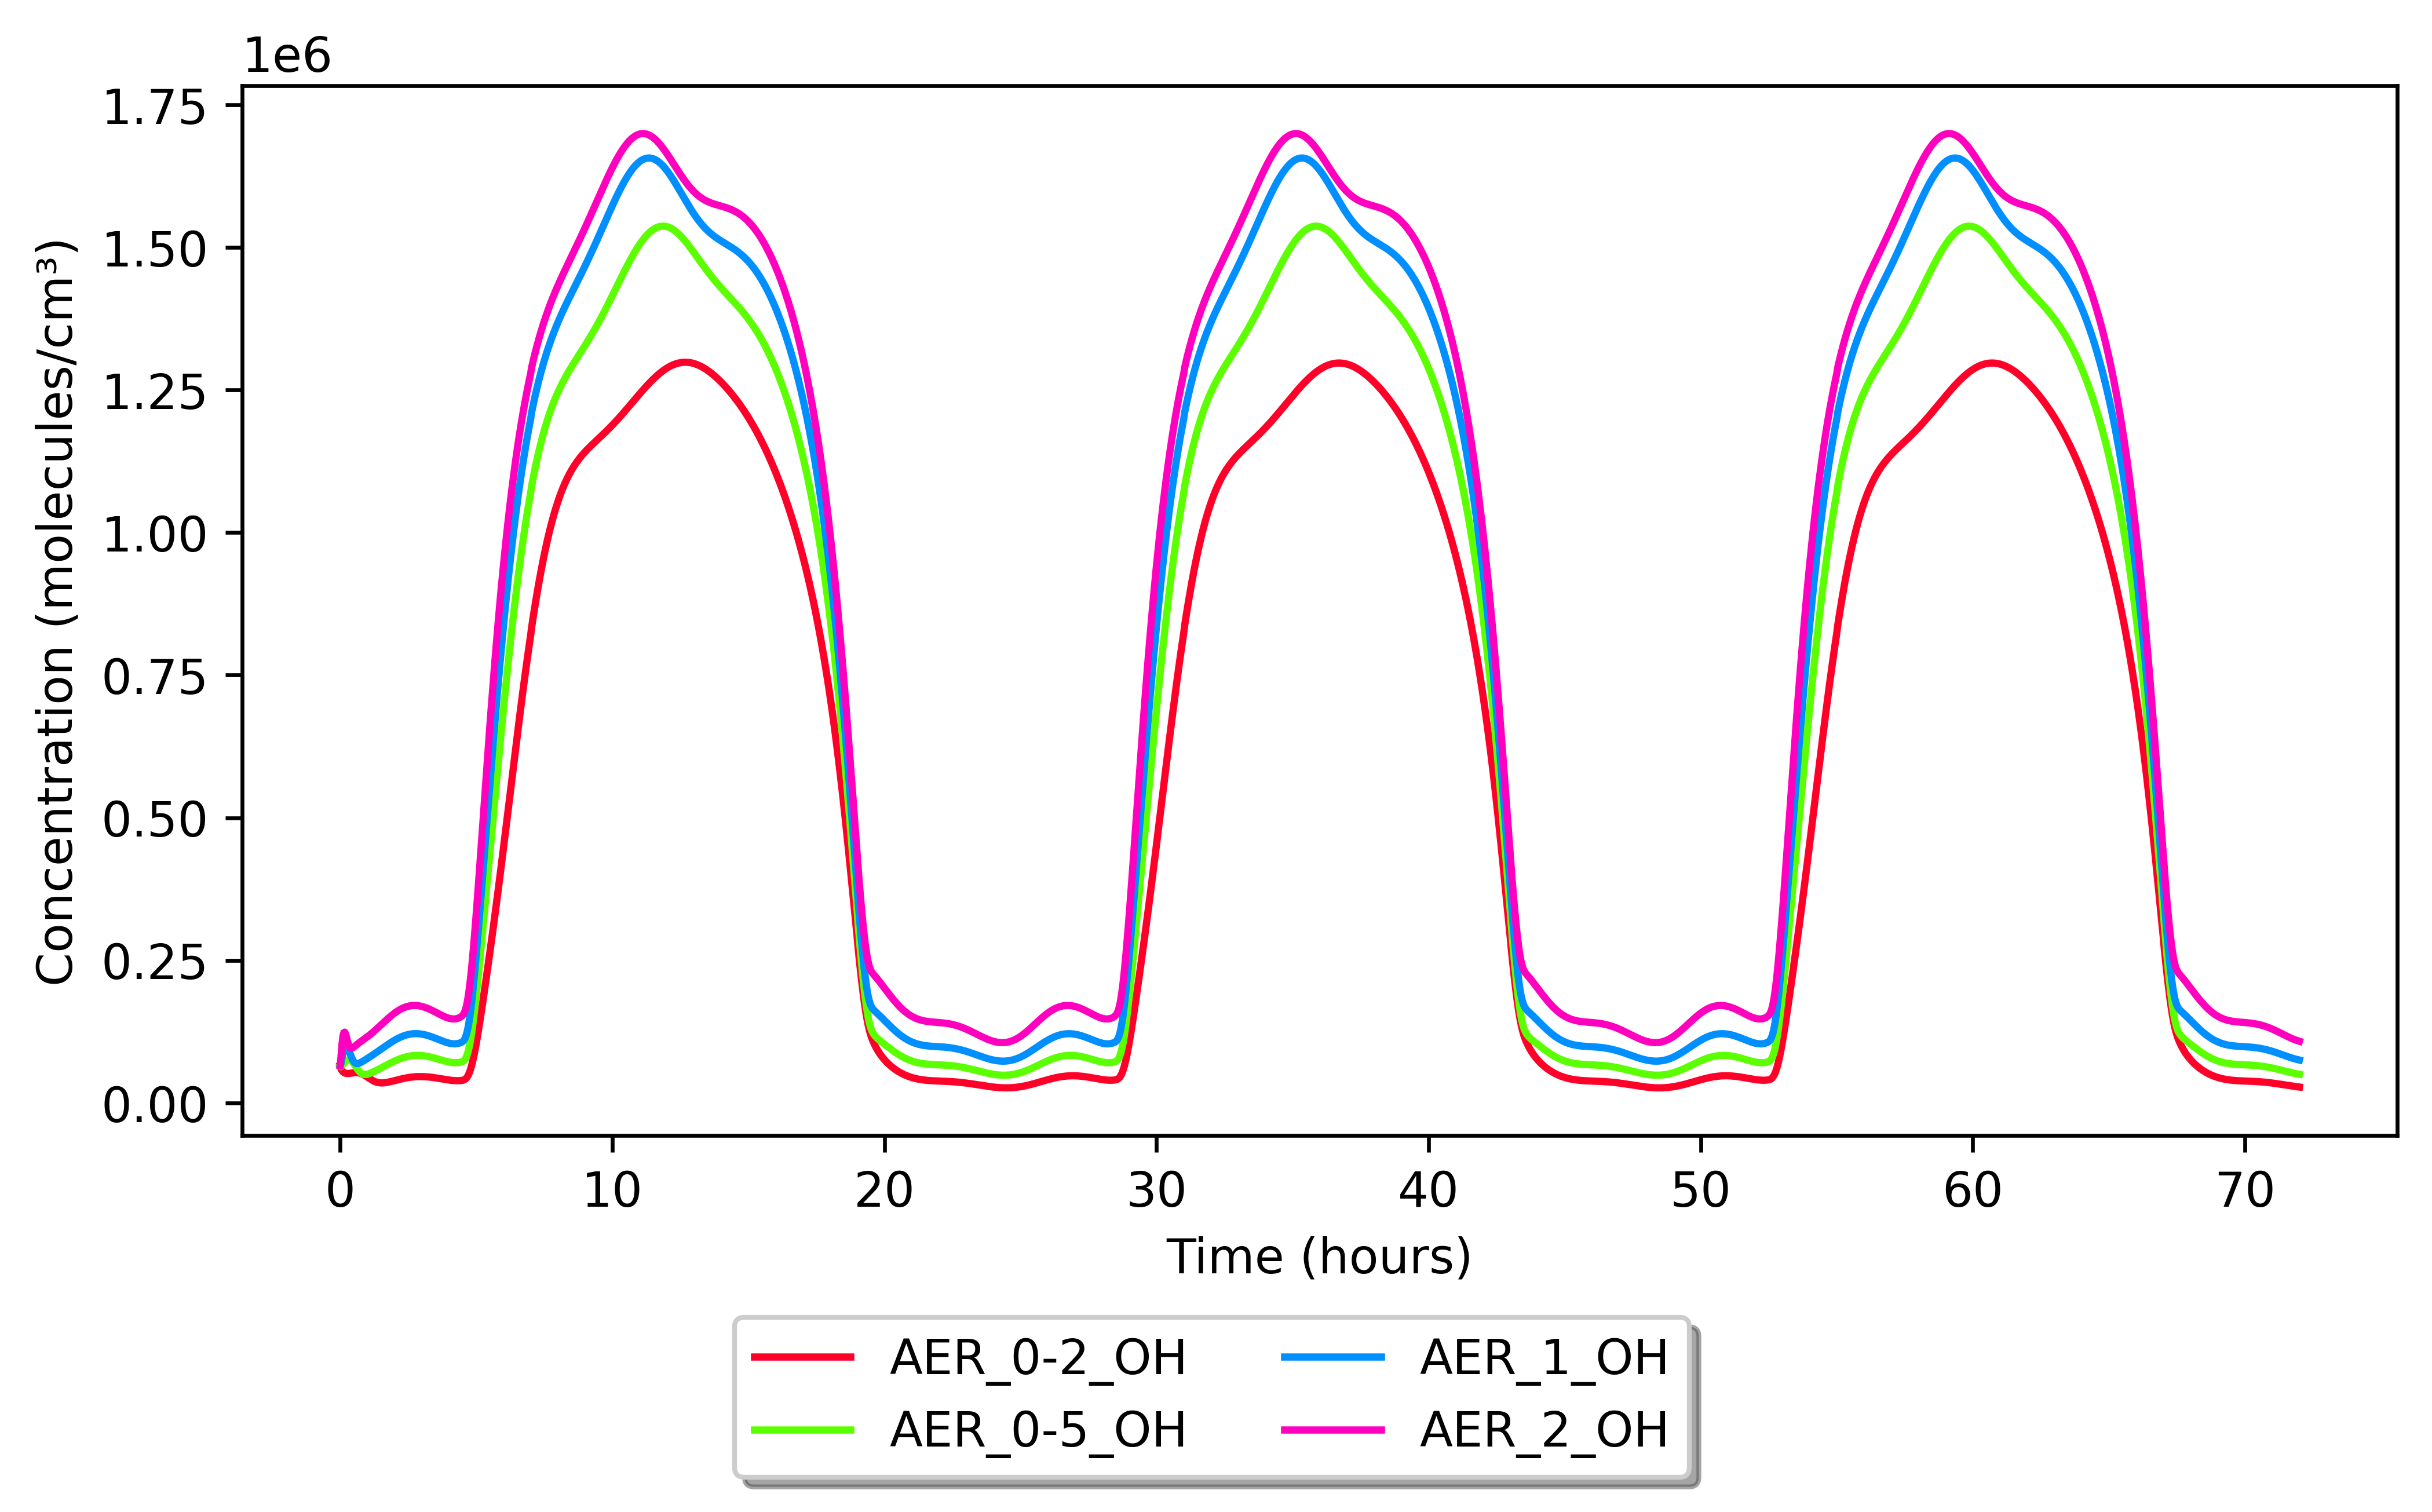
\includegraphics[width=\textwidth]{OH_AER.png}
    \caption{The predicted OH concentrations for AER values of 0.2~h$^{-1}$, 0.5~h$^{-1}$, 1~h$^{-1}$, and 2~h$^{-1}$ with no other variable changes from the INCHEM-Py download default values}
    \label{fig:OH_AER}
\end{figure}



\newpage
\section{Outputs}\label{outputs}\index{outputs}
Multiple files are produced by INCHEM-Py during a model run. The output folder is named automatically using the current date and time in the format \texttt{YYYYMMDD\_hhmmss}, and an additional custom title can be set within the settings.py file. The main output files are listed below: \seealso{\hyperref[settings.py]{settings.py}}

\subsection{settings.py}
A copy of the settings.py file used to run the model.

\subsection{MCM.fac}
A copy of the MCM download used to run the model.

\subsection{out\_data.pickle}\index{out\_data.pickle}
This is the main output of the INCHEM-Py model. This file is a compressed data frame (table) of all of the species concentrations with time. This method (as opposed to outputting all data in the csv format) is used because the data is saved more efficiently and can be opened again in Python for analysis, while retaining the functionality of the data frame when it was saved. Concentrations of species are all in molecules cm$^{-3}$ and follow the naming conventions detailed earlier in this manual.\seealso{\hyperref[Naming conventions]{Naming conventions}}

Included within the output are as follows:
\begin{itemize}
    \item All species concentrations, unless they have been set as constants
    \item The peroxy radical summation "RO2"
    \item Photolysis J values "J1", "J2" etc...
    \item Outdoor concentrations
    \item Reactivity and production rates of species set in  reactivity.py \seealso{\hyperref[reactivity.py]{reactivity.py}}
\end{itemize}
If optional settings are also used, then the following are also included in the output:
\begin{itemize}
    \item Custom summations
    \item Particle concentrations
\end{itemize}

To analyse the output data, there are two approaches. The first is to use inchem\_extractor.py (included in the INCHEM-Py download) which requires little/no working knowledge of Python. The second is to manually extract data from the out\_data.pickle file. Both approaches are outlined below and the choice of which to use depends on the level of analysis required.

\marginlabel{inchem\_extractor.py}\index{inchem\_extractor.py}

A main aim for producing this model was to improve accessibility for use across a wide audience. Therefore, included in the INCHEM-Py download is the inchem\_extractor.py. This provides an easy method of extracting required outputs from model runs that requires little/no prior knowledge of Python. Using this script, all output elements can be extracted from multiple out\_data.pickle files into .csv files and will be plotted for initial assessment of results. A description of this file and its usage is given in appendix \ref{inchem_extractor.py}. 

\marginlabel{Manual data extraction}

For more detailed analysis of the output data, manipulation of the out\_data.pickle file is required. Example commands to import and export the data are shown below. These are necessary if you wish to analyse the data further within Python.

\marginlabel{Importing}
\begin{verbatim}
import pickle
with open("out_data.pickle","rb") as handle:
    out_data=pickle.load(handle)
\end{verbatim}

\marginlabel{Exporting to a csv}
\begin{verbatim}
species_to_export = ["species1", "species2", "species3"]
out_data.to_csv("output.csv", columns = species_to_export)
\end{verbatim}
Although all the data can be exported to a .csv file, the file size will be roughly double that of the equivalent pickle file. 

\subsection{initial\_concentrations.txt}\index{initial\_concentrations, output}
A text file of initial concentrations of all species within the model run at time 0.

\subsection{INCHEM\_inputs.txt}\index{INCHEM\_inputs.txt}
Lists of species, summations, rate coefficents, and reactions included within the additional INCHEM chemistry input file. This file provides a record of the additional indoor reactions used for a particular model run for future reference.

\subsection{master\_array.pickle}\index{master\_array.pickle}
A copy of the master array of ordinary differential equations for all species within the model run. The pickle module in Python can be used to open this to check the build of the ODEs and to investigate the mechanism if required. An example script to load the master array is
\begin{verbatim}
import pickle
    
with open("master_array.pickle", "rb") as handle:
    master_array = pickle.load(handle)
\end{verbatim}


\subsection{jacobian.py}\index{Jacobian}
This script is created by the model and imported again to create the Jacobian (the user cannot edit this file before use). Details of this process can be found later in this document for interested users. \seealso{\hyperref[Jacobian]{Jacobian}}

\subsection{integration\_times.csv}\index{integration\_times.csv}
A CSV of time stamps tracking the time from the start of the model to the start of each integration step. 

\subsection{output.csv (optional)}\index{output.csv}
A CSV table of output species concentrations with time for the species specified in the output\_species variable of settings.py if the output\_graph variable is set to 1.

\subsection{graph.png (optional)}\index{graph.png}
A graph of species concentrations with time for the species specified in the output\_species variable of settings.py. This is only produced if output\_graph = True.

\newpage
\section{Implementations}
\subsection{Time}\index{time}
INCHEM-Py works in local solar time, i.e. it uses a 24 hour period dictated by the location of the Sun in the sky, which is dependent only on the date and the latitude of the location. 

The date input is used to calculate the declination angle of the Sun as
\begin{equation}\index{declination angle}
    dec = -23.45 \times \cos\left(\frac{360}{365.25}\times (d+10)\right)
\end{equation}
where $d$ is the number of days since the start of the year. This accounts for the orbit of the Earth and we can use the solar zenith angle, the angle between the zenith of the location and the solar rays, to account for the rotation of the Earth.

\begin{figure}[ht]
    \centering
    
\includegraphics{solarzenith.png}
    \caption{Diagram of the solar zenith angle}
    \label{fig:solarzenith}
    \index{solar zenith}
\end{figure}
In figure \ref{fig:solarzenith} the solar zenith angle is shown as $\theta$. C denotes the centre of the Earth with the line C to S representing the trace of the solar rays and the line C to Z representing the zenith of the location being modelled. Lat is the latitude of the location and Dec is the declination angle of the Sun. LHA is the local hour angle and is the angle between the meridian of the Sun and the meridian of the location being modelled, it is calculated in radians as
\begin{equation}
    LHA = \left(1+\left(\frac{t}{4.32e4}\right)\right)\times\pi
\end{equation}
where $t$ is the time of day in seconds. With this information, the solar zenith angle can be calculated using some simple trigonometry and the spherical law of cosines as
\begin{multline}
    \cos(\theta) = \cos(90-Lat)\cos(90-Dec)\\
    +\sin(90-Lat)\sin(90-dec)\cos(LHA)
\end{multline}
which simplifies to
\begin{equation}
    \cos(\theta) = \sin(Lat)\sin(Dec)+\cos(Lat)\cos(Dec)\cos(LHA)
\end{equation}

\index{Outdoor concentrations and time}\marginlabel{Outdoor concentrations and time}\label{Outdoor concentrations and time}

No input for longitude is required for these calculations as local solar time will be the same for all latitudes. Therefore, the model must make sure that local outdoor concentrations are also corrected to solar noon if used. Website tools such as \href{https://www.esrl.noaa.gov/gmd/grad/solcalc/}{solcalc} can be used to calculate when solar noon is in local time, from which an adjustment can be made. 

Example 1: My office in York is located at latitude 53.94 and longitude -1.05. On the 12$^{th}$ of November 2020, solar noon was 11:48:24 in local time. Therefore any measurements I made on that day using local time will need to be shifted forward by 11 minutes and 36 seconds for consistency with the calculation of photolysis rates in the model.

Example 2: If you were based in St Lucia at 14.00 degrees latitude and -60.93 degrees longitude on the 5$^{th}$ of May 2018, when solar noon was at 12:00:25 local time, outdoor measurements would need to be shifted 25 seconds back for consistency with the photolysis rate calculations.

The output concentrations from the model are also in local solar time and will need to be converted to local time if to be compared to any measurements taken in local time. For the two examples above, the opposite shift would need to be made. 

Example 3: I run a simulation to compare with experimental data gathered in Nuuk (Greenland) on the 9$^{th}$ of March 2021. Nuuk is at 64.18 degrees latitude and -51.72 degrees longitude with solar noon at 12:44:42 local time. As such I would need to shift the simulated output concentrations forwards by 44 minutes and 42 seconds to put them into local time.

Some outdoor fit calculations (OH, HO$_2$, CH$_3$O$_2$, HONO) use the cosine of the solar zenith angle (labelled as 'cosx' in the outdoor photolysis rate calculations in the model, $\cos(\theta)$ in equations (3) and (4) above) and thus are already in local solar time.

\index{horizon}\marginlabel{The horizon}

The model uses a horizon at 90$^{\circ}$ to the zenith (the astronomical horizon). Any simulation where the declination of the Sun plus the latitude is over 90$^{\circ}$ or below -90$^{\circ}$ will have the Sun below the horizon. This does not mean the location cannot be simulated, simply that the location will have no sunlight. At its maximum, the solar declination angle is $\pm$23.45$^{\circ}$ meaning that locations beyond $\pm$66.55$^{\circ}$ (within the Arctic or Antarctic circle) will have no sunlight at this time.

\subsection{Integration}\index{Integration}\label{Integration}
INCHEM-Py uses \hyperlink{https://docs.scipy.org/doc/scipy/reference/generated/scipy.integrate.ode.html}{scipy.integrate.ode} which is a class that gives access to various numerical integrators. Due to the stiff and highly coupled nature of the system, LSODA from the Fortran solver package \hyperlink{http://www.netlib.org/odepack/}{ODEPACK} is used \cite{Hindmarsh1983}. 

The default integrator arguments set within INCHEM-Py are as follows:
\begin{itemize}
    \item \texttt{atol = [1e-6]*num\_species}\\
    The absolute tolerance for solution. "num\_species" is the total number of species.
    \item \texttt{rtol = 1e-6}\\
    The relative tolerance for solution.
    \item \texttt{first\_step = 1e-10}\\
    The size of the first integration step to try (s).
    \item \texttt{nsteps = 5000}\\
    The maximum number of internal time steps allowed.
\end{itemize}

\marginlabel{return code}\index{return code}

The integrator will report a return code to the console when it has stopped running. This could be to say that the integration was successful or it might report an error if the integration has failed. The return codes are as follows:

2 - Integration successful.\\
-1 - Excess work done on this call (perhaps wrong Dfun type).\\
-2 - Excess accuracy requested (tolerances too small).\\
-3 - Illegal input detected (internal error).\\
-4 - Repeated error test failures (internal error).\\
-5 - Repeated convergence failures (perhaps bad Jacobian or tolerances).\\
-6 - Error weight became zero during problem.\\
-7 - Internal workspace insufficient to finish (internal error).

The return codes can point to any number of issues with the model which are too numerous to go through in this manual. If changes have only been made to the settings.py file then the most likely failure would be due to timed emissions causing fast changes in species concentrations. The integrator may then not being able to reach the next time step within "nsteps" due to the small internal time steps required to resolve these fast reactions. The solution to this is to either consider whether the input emission rates are too high or to decrease "dt" in settings.py to give the integrator a shorter interval to integrate over.


\marginlabel{threadpoolctl}

During integration the model will attempt to use multiple threads. To stop this using all available resources of the computer, threadpoolctl is used. \texttt{threadpool\_limits(limit=4)} keeps the simulation using a maximum of 4 threads.


\subsection{Outdoor concentrations}\label{outdoor_concentrations.py}\index{Outdoor concentrations}
Outdoor concentrations are set in one of two ways. Most simply, the user can set a constant outdoor value for a species. The user can refer to the outdoor\_concentrations.py module to see which concentrations are already set and to which values. To add a new outdoor species, simply  take the name of the species you wish to have an outdoor concentration of, add "OUT" to the end of it, and add an entry into the dictionary with a concentration in molecules cm$^{-3}$. If they do not appear in the outdoor dictionary, the outdoor concentration is 0.

It is also possible to define a diurnal profile for outdoor concentrations. For OH, HO$_2$, CH$_3$O$_2$, and HONO, concentrations are calculated with dependency on the solar zenith angle\seealso{\hyperref[Outdoor concentrations and time]{Outdoor concentrations and time}}. Diurnal outdoor concentrations for O$_3$, NO$_2$, NO, and PM 2.5 (TSPOUT) have been been obtained from fits to measurements from four European locations. We have included three profiles from data measured in 2018 for different types of location. This data was downloaded from the \href{https://aqportal.discomap.eea.europa.eu/products/data-viewers/statistical-viewer-expert/}{European air quality database} for the following background stations:
\begin{itemize}
    \item GB0566A, urban London, -0.125889	51.52229
    \item GB0586A, suburban London, 0.070766	51.45258
    \item NO0120A, urban Bergen, 5.312674	60.395929
\end{itemize} 
The downloaded data for these three locations is provided as hourly averages, with a start time and an end time. A midpoint time was set and then shifted from local time, given in UTC, to solar time using the station longitude. The solar shift varies daily and should be calculated for each time. Quarter three data (July, August, September) was then extracted from the year and daily measurements overlaid. Hourly averages of both the time and the concentration were used to fit the trigonometric Fourier functions which are included in INCHEM-Py. 

A fourth city, Milan, is also included, based on Terry et al. (2014) \cite{Terry2014}. This data is from a particularly polluted two week period in Milan in August 2003. The raw data for the 2 week period was averaged to a 24 hour period and a trigonometric Fourier function fit compiled. 

Additional fits to locations can be added to the outdoor\_concentrations.py file in the diurnal function following the format given within the file. These functions use n for the time value as a repeating time series between 0 and 86400 s. The process of extracting, averaging, and fitting raw outdoor measured data is not trivial and requires decisions about handling raw data which is not for us to prescribe. We can provide advice and assistance if required.

Calculating diurnal concentrations outdoors is optional. If the user defines constant outdoor averages and also diurnally varying outdoor concentrations, the latter will take precedence as they are calculated second by the model. Outdoor concentrations are set as inputs, the model does not update outdoor values based on transfer from indoors.

To help choose which outdoor concentration might be best for your purposes, plots of outdoor concentrations fits from the different locations are shown in appendix \ref{outdoor_fits}.

\subsection{Photolysis}\label{photolysis.py}
Photolysis in INCHEM-Py is calculated for both indoor light sources and sunlight entering from outdoors. These values are then summed and used as a total photolysis rate for photolysis reactions. The following photolysis coefficients are calculated with the corresponding species or species group:

\begingroup
\allowdisplaybreaks
\begin{flalign*}
J1&:    O_3 \rightarrow O(^1D) + O_2\\
J2&:    O_3\rightarrow O(^3P)+O_2\\
J3&:	H_2O_2 \rightarrow OH + OH\\
J4&:	NO_2 \rightarrow NO + O(^3P)\\
J5&:	NO_3 \rightarrow NO + O_2\\
J6&:	NO_3 \rightarrow NO_2 + O(^3P)\\
J7&:	HONO \rightarrow NO+OH\\
J8&:	HNO_3 \rightarrow NO_2 + OH\\
J11&:	HCHO \rightarrow H+HCO\\
J12&:	HCHO \rightarrow H_2+CO\\
J13&:	CH_3CHO \rightarrow CH_3 + HCO\\
J14&:	C_2H_5CHO \rightarrow C_2H_5 + HCO\\
J15&:	C_3H_7CHO\rightarrow C_3H_7 + HCO\\
J16&:	C_3H_7CHO\rightarrow C_2H_4 + CH_3CHO\\
J17&:	IPRCHO \rightarrow C_4H_9 + HCO\\
J18&:	MACR \rightarrow CH_2=CCH_3+HCO\\
J19&:	MACR\rightarrow CH_2=C(CH_3)CO+H\\
J20&:	C_5H_8O_3\rightarrow CH_3C(CHO)=CHCH_2O+OH\\
J21&:	CH_3C(O)CH_3\rightarrow CH_3CO + CH_3\\
J22&:	MEK\rightarrow CH_3CO+C_2H_5\\
J23&:	MVK\rightarrow CH_3CH=CH_2 + CO\\
J24&:	MVK\rightarrow CH_3CO + CH_2=CH\\
J31&:	GLYOX\rightarrow CO + CO + H_2\\
J32&:	GLYOX\rightarrow HCHO + CO\\
J33&:	GLYOX\rightarrow HCO + HCO\\
J34&:	MGLYOX\rightarrow CH_3CO + HCO\\
J35&:	BIACET\rightarrow CH_3CO + CH_3CO\\
J41&:	CH_3OOH\rightarrow CH_3O + OH\\
J51&:	CH_3ONO_2\rightarrow CH_3O + NO_2\\
J52&:	C_2H_5ONO_2\rightarrow C_2H_5O + NO_2\\
J53&:	n-C_3H_7ONO_2\rightarrow n-C_3H_7O + NO_2\\
J54&:	i-C_3H_7ONO_2\rightarrow CH_3C(O)CH_3 + NO_2\\
J55&:	t-C_4H_9NO_3\rightarrow t-C_4H_9O + NO_2\\
J56&:	NOA\rightarrow CH_3C(O)CH_2(O)+NO_2\\
J57&:	NOA\rightarrow CH_3CO+HCHO+NO_2\\
J70&:	Cl_2\rightarrow Cl+Cl\\
J71&:	ClNO_2\rightarrow NO_2+Cl\\
J72&:	ClONO_2\rightarrow NO_3+Cl\\
J73&:	ClONO_2\rightarrow NO_2+Cl\\
J74&:	HOCl\rightarrow OH+Cl\\
J75&:	OClO\rightarrow O+ClO\\
J76&:	ClO\rightarrow O+Cl\\
J77&:	ClOOCl\rightarrow ClOO+Cl\\
J78&:	ClOOCl\rightarrow ClO+ClO\\
\end{flalign*}
\endgroup

The absorption cross-section of a species, or group of species, is wavelength dependant. For INCHEM-Py, the wavelengths of multiple light sources, and the transmission factor of wavelengths through multiple glass types have been used to calculate the photolysis coefficients 1 m away from these sources of light. Full details of this process can be found in Wang et al. (in preparation, 2021) \cite{Wang2021}. 

The light types (input parameter) are shown below. Details of these lights for calculating the photolysis rates were taken from Kowal et al. (2017) \cite{Kowal2017}.
\begin{itemize}
    \item Incandescent ("Incand")
    \item Halogen ("Halogen")
    \item Light emitting diode ("LED")
    \item Compact fluorescent lamps ("CFL")
    \item Uncovered fluorescent tube ("UFT")
    \item Covered fluorescent tube ("CFT")
    \item Fluorescent tube ("FT")
\end{itemize}

The glass types, wavelength range (input parameters) are shown below. The transmittance of these different glass types were taken from Blocquet et al. (2018) \cite{Blocquet2018}.
\begin{itemize}
    \item Glass C Sacht self-cleaning, 315-700~nm ("glass\_C")
    \item Low emissivity, 330-700~nm ("low\_emissivity")
    \item Low emissivity with film, 380-700~nm ("low\_emissivity\_film")
\end{itemize}

\subsection{Surface deposition}\label{surface_dictionary.py}
The HMIX variable represents the surface to volume (A/V) ratio of a given space. Within the surface dictionary, the deposition velocities are multiplied by HMIX and then fed to the ODE for each species. Particles are assigned a deposition velocity of 0.004 cm s$^{-1}$ with other species, as described in Carslaw et al. (2012) \cite{Carslaw2012}. Species that do not have a value within the surface dictionary are given a deposition velocity of 0 and do not deposit. Deposition of any new species can be added in the custom\_input.txt file as a reaction with the rate coefficient of the deposition velocity. 
\begin{verbatim}
0.016*HMIX : species1 =
\end{verbatim}


\subsection{Additonal INCHEM reactions}\label{inchem_chemistry}
To analyse varying scenarios indoors, additional chemistry mechanisms have been developed by Carslaw and coworkers, and can be included within INCHEM-Py if required. These schemes are not fully explicit as per the MCM. They typically use the rate coefficients for the preliminary oxidation steps using data from the literature and then map onto existing MCM species after a few degradation steps where relevant, to reduce additional complexity. The following species have been treated in this way:
\begin{itemize}
    \item Linalool \cite{Carslaw2017}
    \item Octanal, nonanal, decanal \cite{Kruza2017}
    \item Chlorine \cite{Xue2015,Wong2017,Wang2020}, photolysis J70-J74 from \href{http://iupac.pole-ether.fr}{iupac}
    \item Camphene, carene, terpinene \cite{Carslaw2007}
    \item Lactic acid
\end{itemize}

This chemistry is included in the inchem\_chemistry.py module and careful modification is possible but we ask that any additional chemistry is added using the custom\_inputs.txt file as detailed in section \ref{custom_input.txt}. The chemistry is stored in the following format that any modification should follow:

\marginlabel{Peroxy radical species}
These species are peroxy radicals to be added to the peroxy radical summation. They are not species included in the MCM.
\begin{verbatim}
INCHEM_RO2 = ["species1","species2"]
\end{verbatim}

\marginlabel{Summations}
These summations are summations used in reactions or rate coefficients within the INCHEM additional chemistry.
\begin{verbatim}
INCHEM_sums = [["sum_name","species1 + species2 + species3"],
              ["sum_name2","species4 + species5 + species6"]]
\end{verbatim}

\marginlabel{Rate coefficients}
These are generic rate coefficients used in the INCHEM additional chemistry.
\begin{verbatim}
INCHEM_rates=[
["name","rate coefficient calculation"],
["name2","rate coefficient calculation"]
]
\end{verbatim}

\marginlabel{Reactions}
These are the INCHEM additional chemistry reactions and their rate coefficients.
\begin{verbatim}
INCHEM_reactions=[
["rate coefficient calculation","species1 + species2 = species3"],
["rate coefficient calculation","species4 = species5 + species6"]
]
\end{verbatim}

All generic rate coefficients, species and summations can be called in any additional reactions or summations added to the custom\_inputs.txt file.

\subsection{Master array and Jacobian}
\index{master array}\marginlabel{Master array}
The master array is a dictionary of species and their ordinary differential equations (ODEs) that are processed by the integrator. The ODEs are constructed from the reactions input from the MCM, the INCHEM chemistry input file, any custom reactions added via the custom inputs file, and the gas-to-particle reactions. 

To compute the ODEs the reactions must be parsed. Each reaction comprises of a reaction equation and a rate coefficient. For example:
\begin{equation*}
\begin{split}
    y_1 + y_2 &\xrightarrow[]{k_1} y_3 + y_4\\
    y_2 + y_3 &\xrightarrow[]{k_2} y_1
\end{split}
\end{equation*}
where $y_n$ represents the species concentration. In the first reaction all species change at a rate of $y_1y_2k_1$ and in the second reaction all species change at a rate of $y_2y_3k_2$. The change is either positive or negative, depending on which side of the reaction they are on. The code splits the reaction into loss species (1, 2 and 3) and gain species (1, 3, and 4) and assigns a negative reaction to the ODE of species in the list of loss species, and a positive reaction to the ODE of species in the list of gain species. Therefore the following is obtained:
\begin{equation*}
\begin{split}
    &\frac{dy_1}{dt} = y_2y_3k_2 - y_1y_2k_1\\
    &\frac{dy_2}{dt} = - y_1y_2k_1 - y_2y_3k_2\\
    &\frac{dy_3}{dt} = y_1y_2k_1 - y_2y_3k_2\\
    &\frac{dy_4}{dt} = y_1y_2k_1
\end{split}
\end{equation*}
This is repeated for all reactions input into the model. On top of the terms from reactions there are extra terms for air exchange, surface deposition, and any timed emission changes that are defined in the settings file.

This series of ODEs is the master array and is used to construct the Jacobian and reactivity and production functions. The dictionary is also saved to the output folder so that users may analyse the ODEs should they wish.

\index{Jacobian}\marginlabel{Jacobian}\label{Jacobian}

The Jacobian is built in a two stage process.

Stage one is parsing the master array. Each ODE is differentiated with respect to each species in the simulation and a script is written to the output folder. This script contains each dy/dy equation, in string form with a compile instruction, shown alongside index positions for the Jacobian matrix.

The created function is then imported back into the model and run to create the Jacobian matrix from the index positions and compiled equations.

\subsection{Timed emissions}\index{timed emissions}\label{timed emissions, implementation}
Timed emissions are implemented in the settings.py file. \seealso{\hyperref[settings.py]{settings.py}} When writing the master array, a term is included in every ODE for a timed emission. This is 0 unless specified in the settings.py file. When specified, INCHEM-Py will set the timed term in the master array to the given rate when the time step of the simulation is between the user entered start and end time. 

Typical use of this function is to input an event into the model where there may be an emission of a species, such as through cleaning. An example for a limonene input is shown below with a sample result in figure \ref{fig:timed_limonene}. 

\begin{verbatim}
timed_inputs = {"LIMONENE":[[36720,37320,5e8]]}    
\end{verbatim}

Multiple species can be input as:
\begin{verbatim}
timed_inputs = {"LIMONENE":[[36720,37320,5e8]],
                "APINENE":[[36720,37320,5e8]]}
\end{verbatim}

A single species can be input at multiple times as:
\begin{verbatim}
timed_inputs = {"LIMONENE":[[36720,37320,5e8],[39000,39400,5e8]]} 
\end{verbatim}

\clearpage
\begin{figure}[h!]
    \centering
    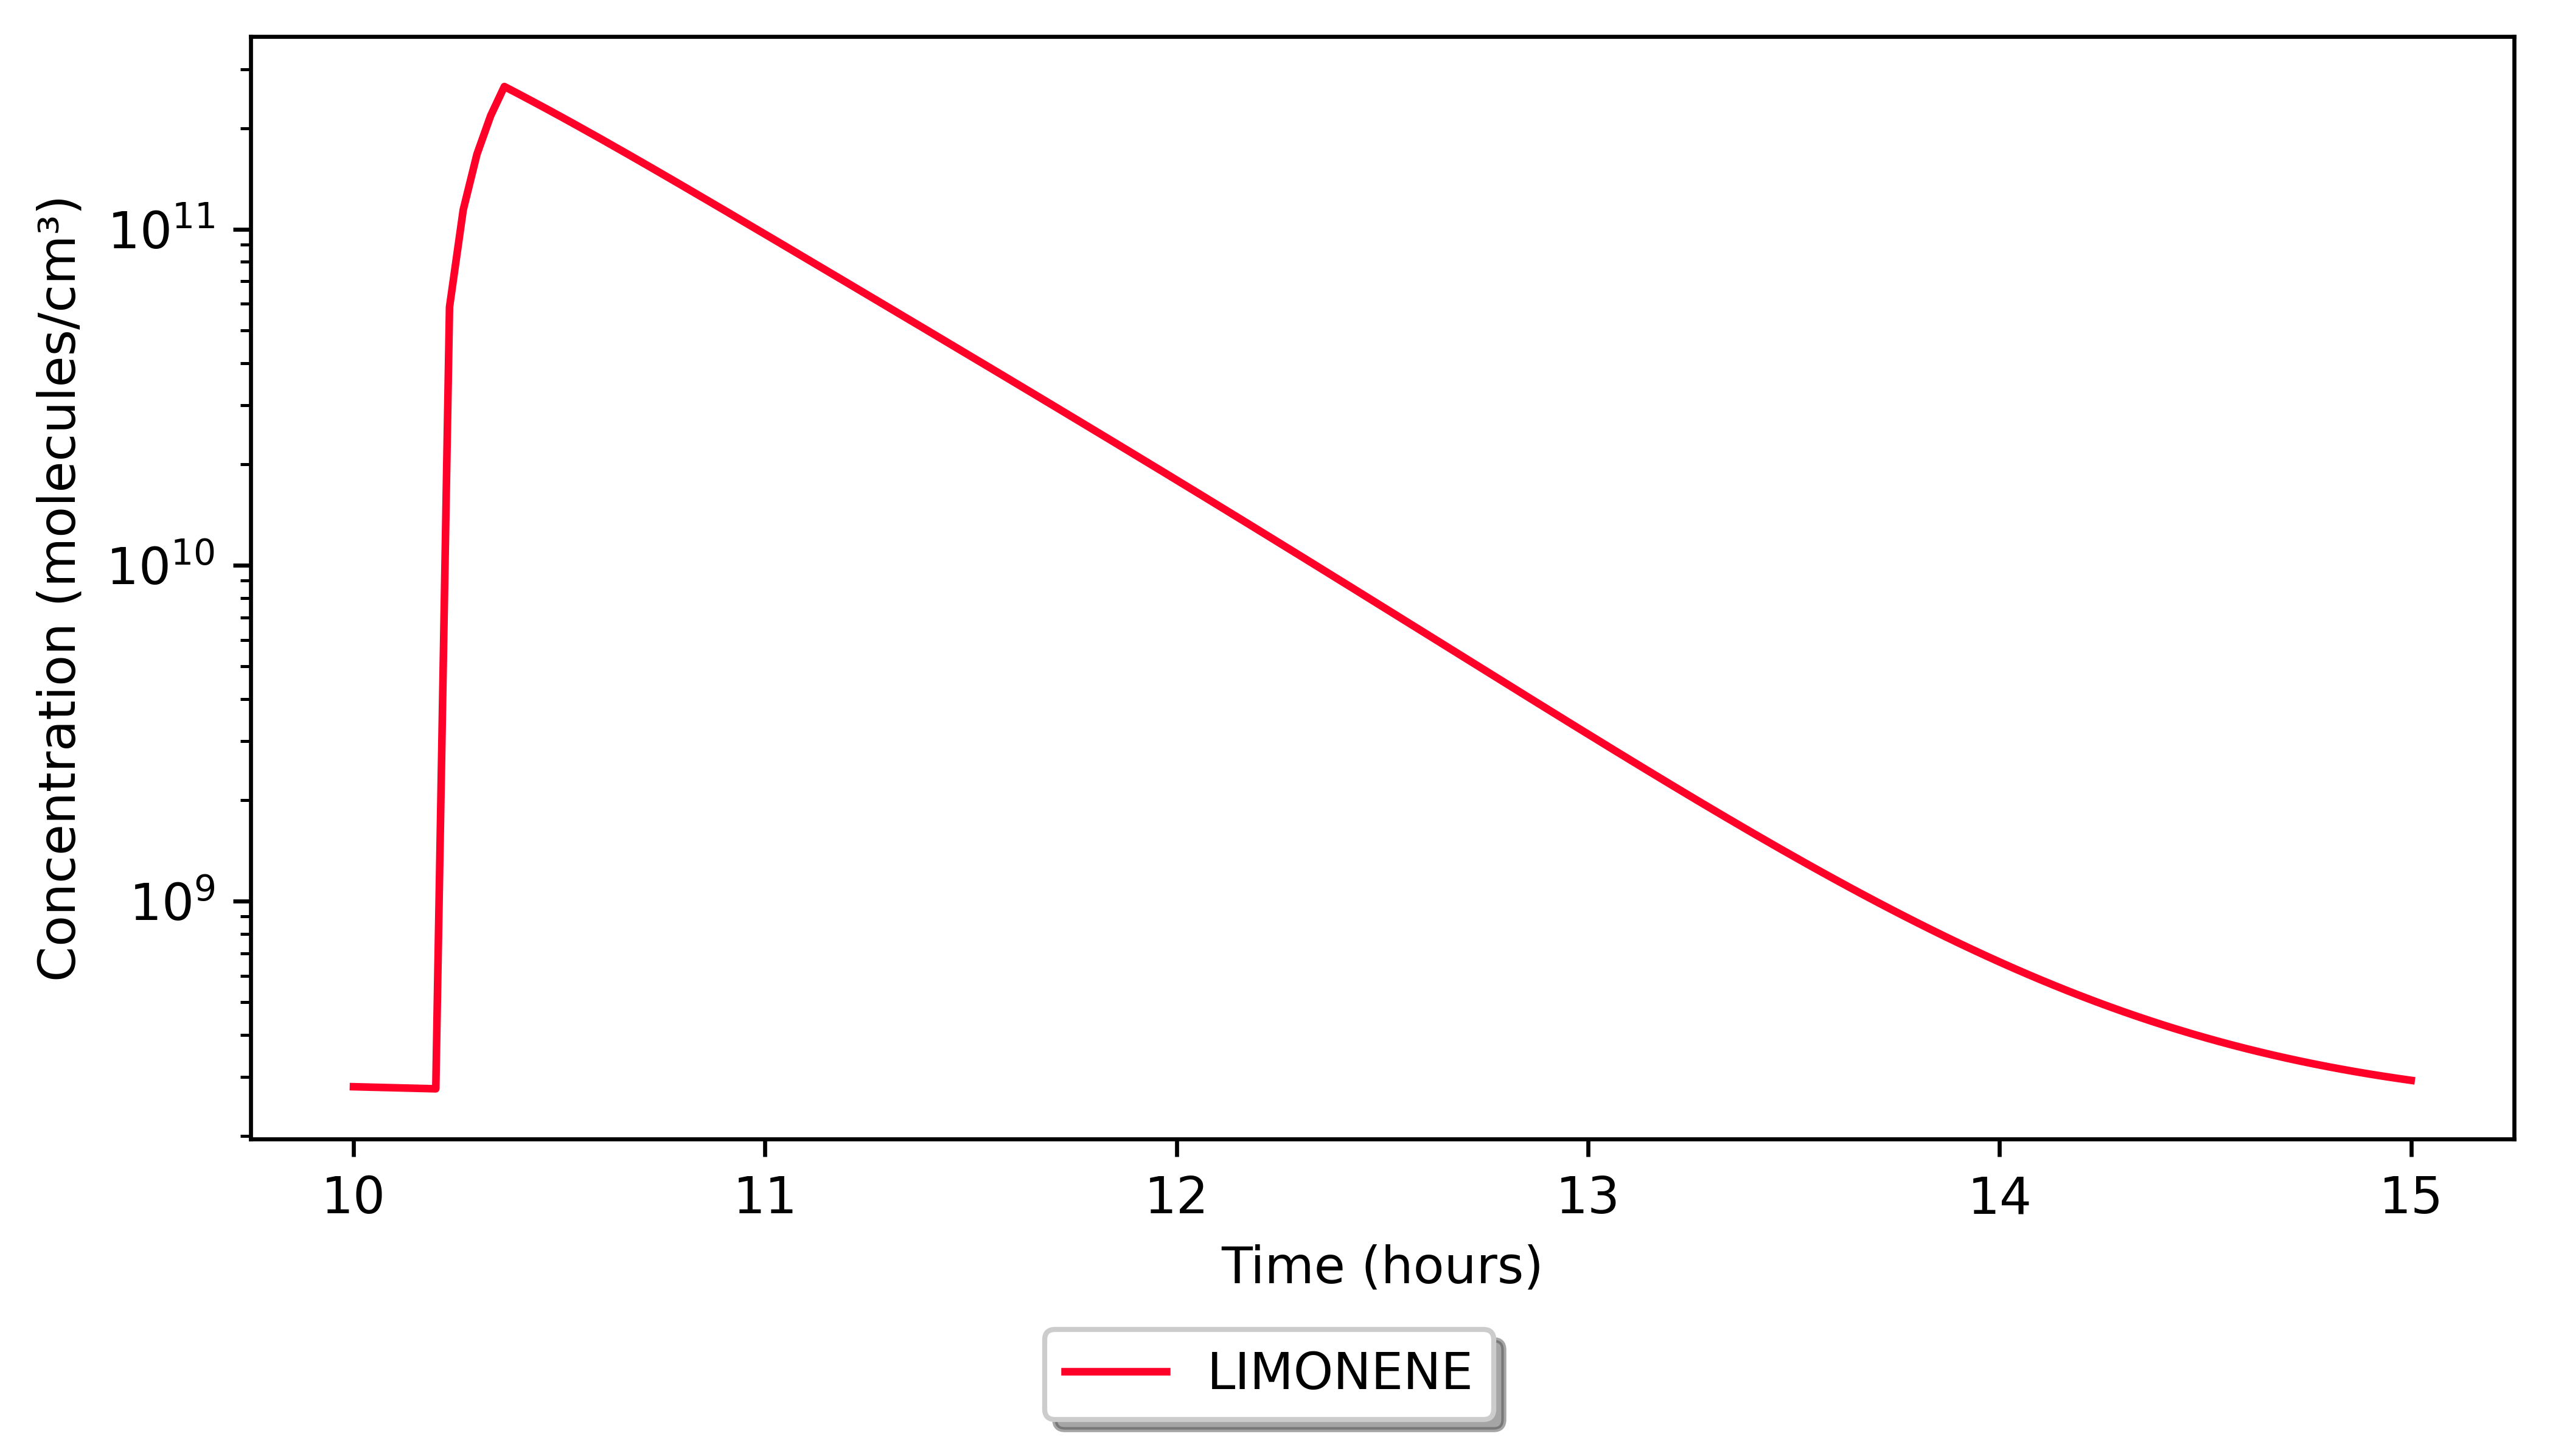
\includegraphics[width=\textwidth]{timed_limonene.png}
    \caption{Limonene timed to increase for 5 minutes at a rate of $5\times10^8$ molecules s$^{-1}$}
    \label{fig:timed_limonene}
\end{figure}

\subsection{Reactivity and production}\index{reactivity}\index{production}\label{reactivity.py}
The reactivity.py file contains functions to calculate the total reactivity and total production rates of selected species included in the "reactivity\_species" list in the reactivity\_summation function (default only OH). The total reactivity of a species, $x$, is the inverse of the lifetime of $x$ and is calculated by summing the reactivity of all other species with $x$. The production rate of a species is a summation of all of the reaction rates that create the species. Reactivity is in units of s$^{-1}$ and production is in units of molecules cm$^{-3}$ s$^{-1}$.

Additional species reactivity and production values can be added by adding the species in question to the reactivity\_species list within the reactivity.py module. By default it is set to only include OH.
\begin{verbatim}
    reactivity_species = ['OH']
\end{verbatim}

\section{Community}
We welcome any contributions to INCHEM-Py and look forward to working with a community of people to develop the model further. 

Please contact us if you require any support.\\
david.shaw@york.ac.uk\\
nicola.carslaw@york.ac.uk

INCHEM-Py is free software, but since it is a scientific code we also ask that you show professional courtesy when using this code:
\begin{enumerate}
    \item Since you are benefiting from work on INCHEM-Py, we ask that you submit any improvements you make to the code to us by submitting a pull request. Issues should be reported using the issue tracker (\url{https://github.com/DrDaveShaw/INCHEM-Py/issues}).
    \item If you use INCHEM-Py results in a paper or professional publication, we ask that it includes an appropriate reference. It is understood that in most cases if one or more of the INCHEM-Py team are involved in preparing results then they should appear as co-authors.
    \item The INCHEM-Py logo is included with the model and may optionally be used in any oral or poster presentations.
\end{enumerate}

\subsection{Acknowledgements}
The development of this model has been funded by a grant from the Alfred P. Sloan Foundation, grant number 2018-10083. Conclusions reached or positions taken by researchers or other grantees represent the views of the grantees themselves and not those of the Alfred P. Sloan Foundation or its trustees, officers, or staff. 

The authors would like to thank Magdalena Kruza, Freja Oesterstroem, Helen Davies, Zixu Wang, Georgia Beel, Ellen Harding-Smith, Toby Carter and Michael Cooper for their assistance and feedback during model development. We would also like to thank Ramsay Carslaw for the initial design of the model logo.

%%%%%%%%%%%%%%%%%%%%%%%%%%%%%%%%%%%%%%%%%%%%%%%%%%%%%%%%%%%%%%%%%%%%%%

\printindex

\printbibliography

\newpage
\appendix
\section{Outdoor concentrations}\label{outdoor_fits}
\begin{figure}[h!]
    \centering
    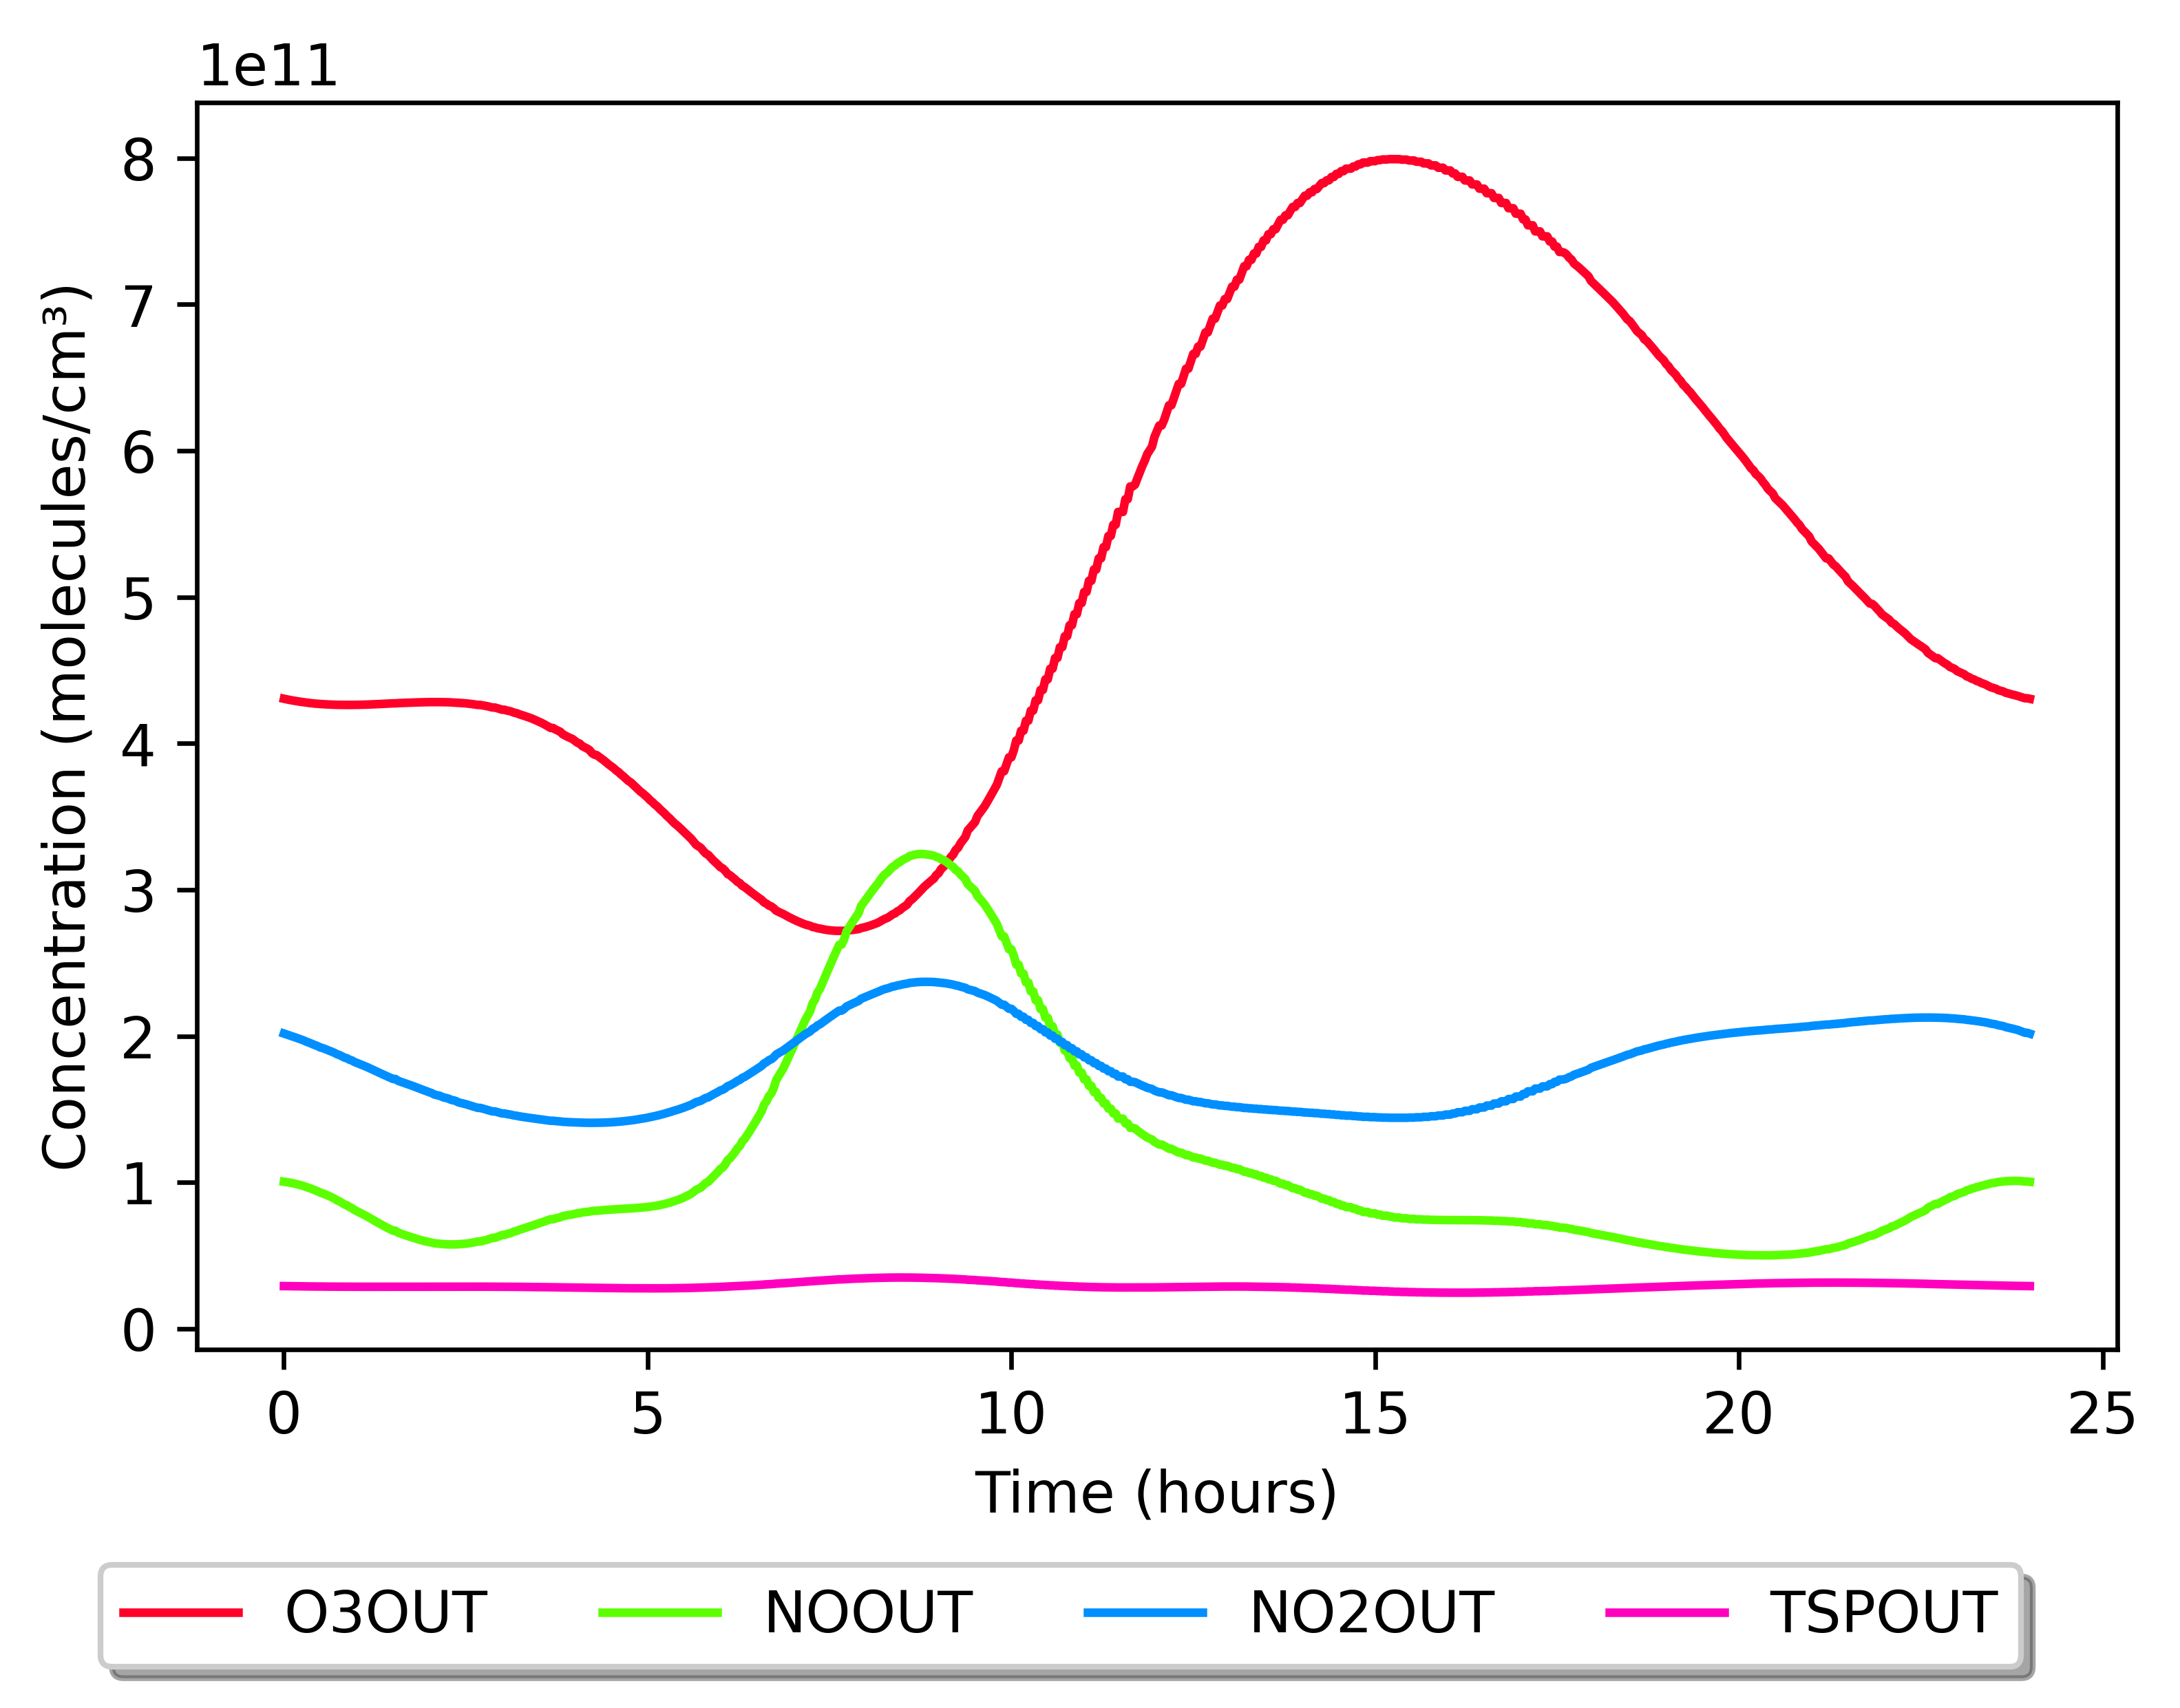
\includegraphics[width=\textwidth]{London_urban.png}
    \caption{Outdoor average concentration fits for GB0566A, urban London, Q3 2018.}
    \label{fig:Out_lon_urb}
\end{figure}
\begin{figure}[h!]
    \centering
    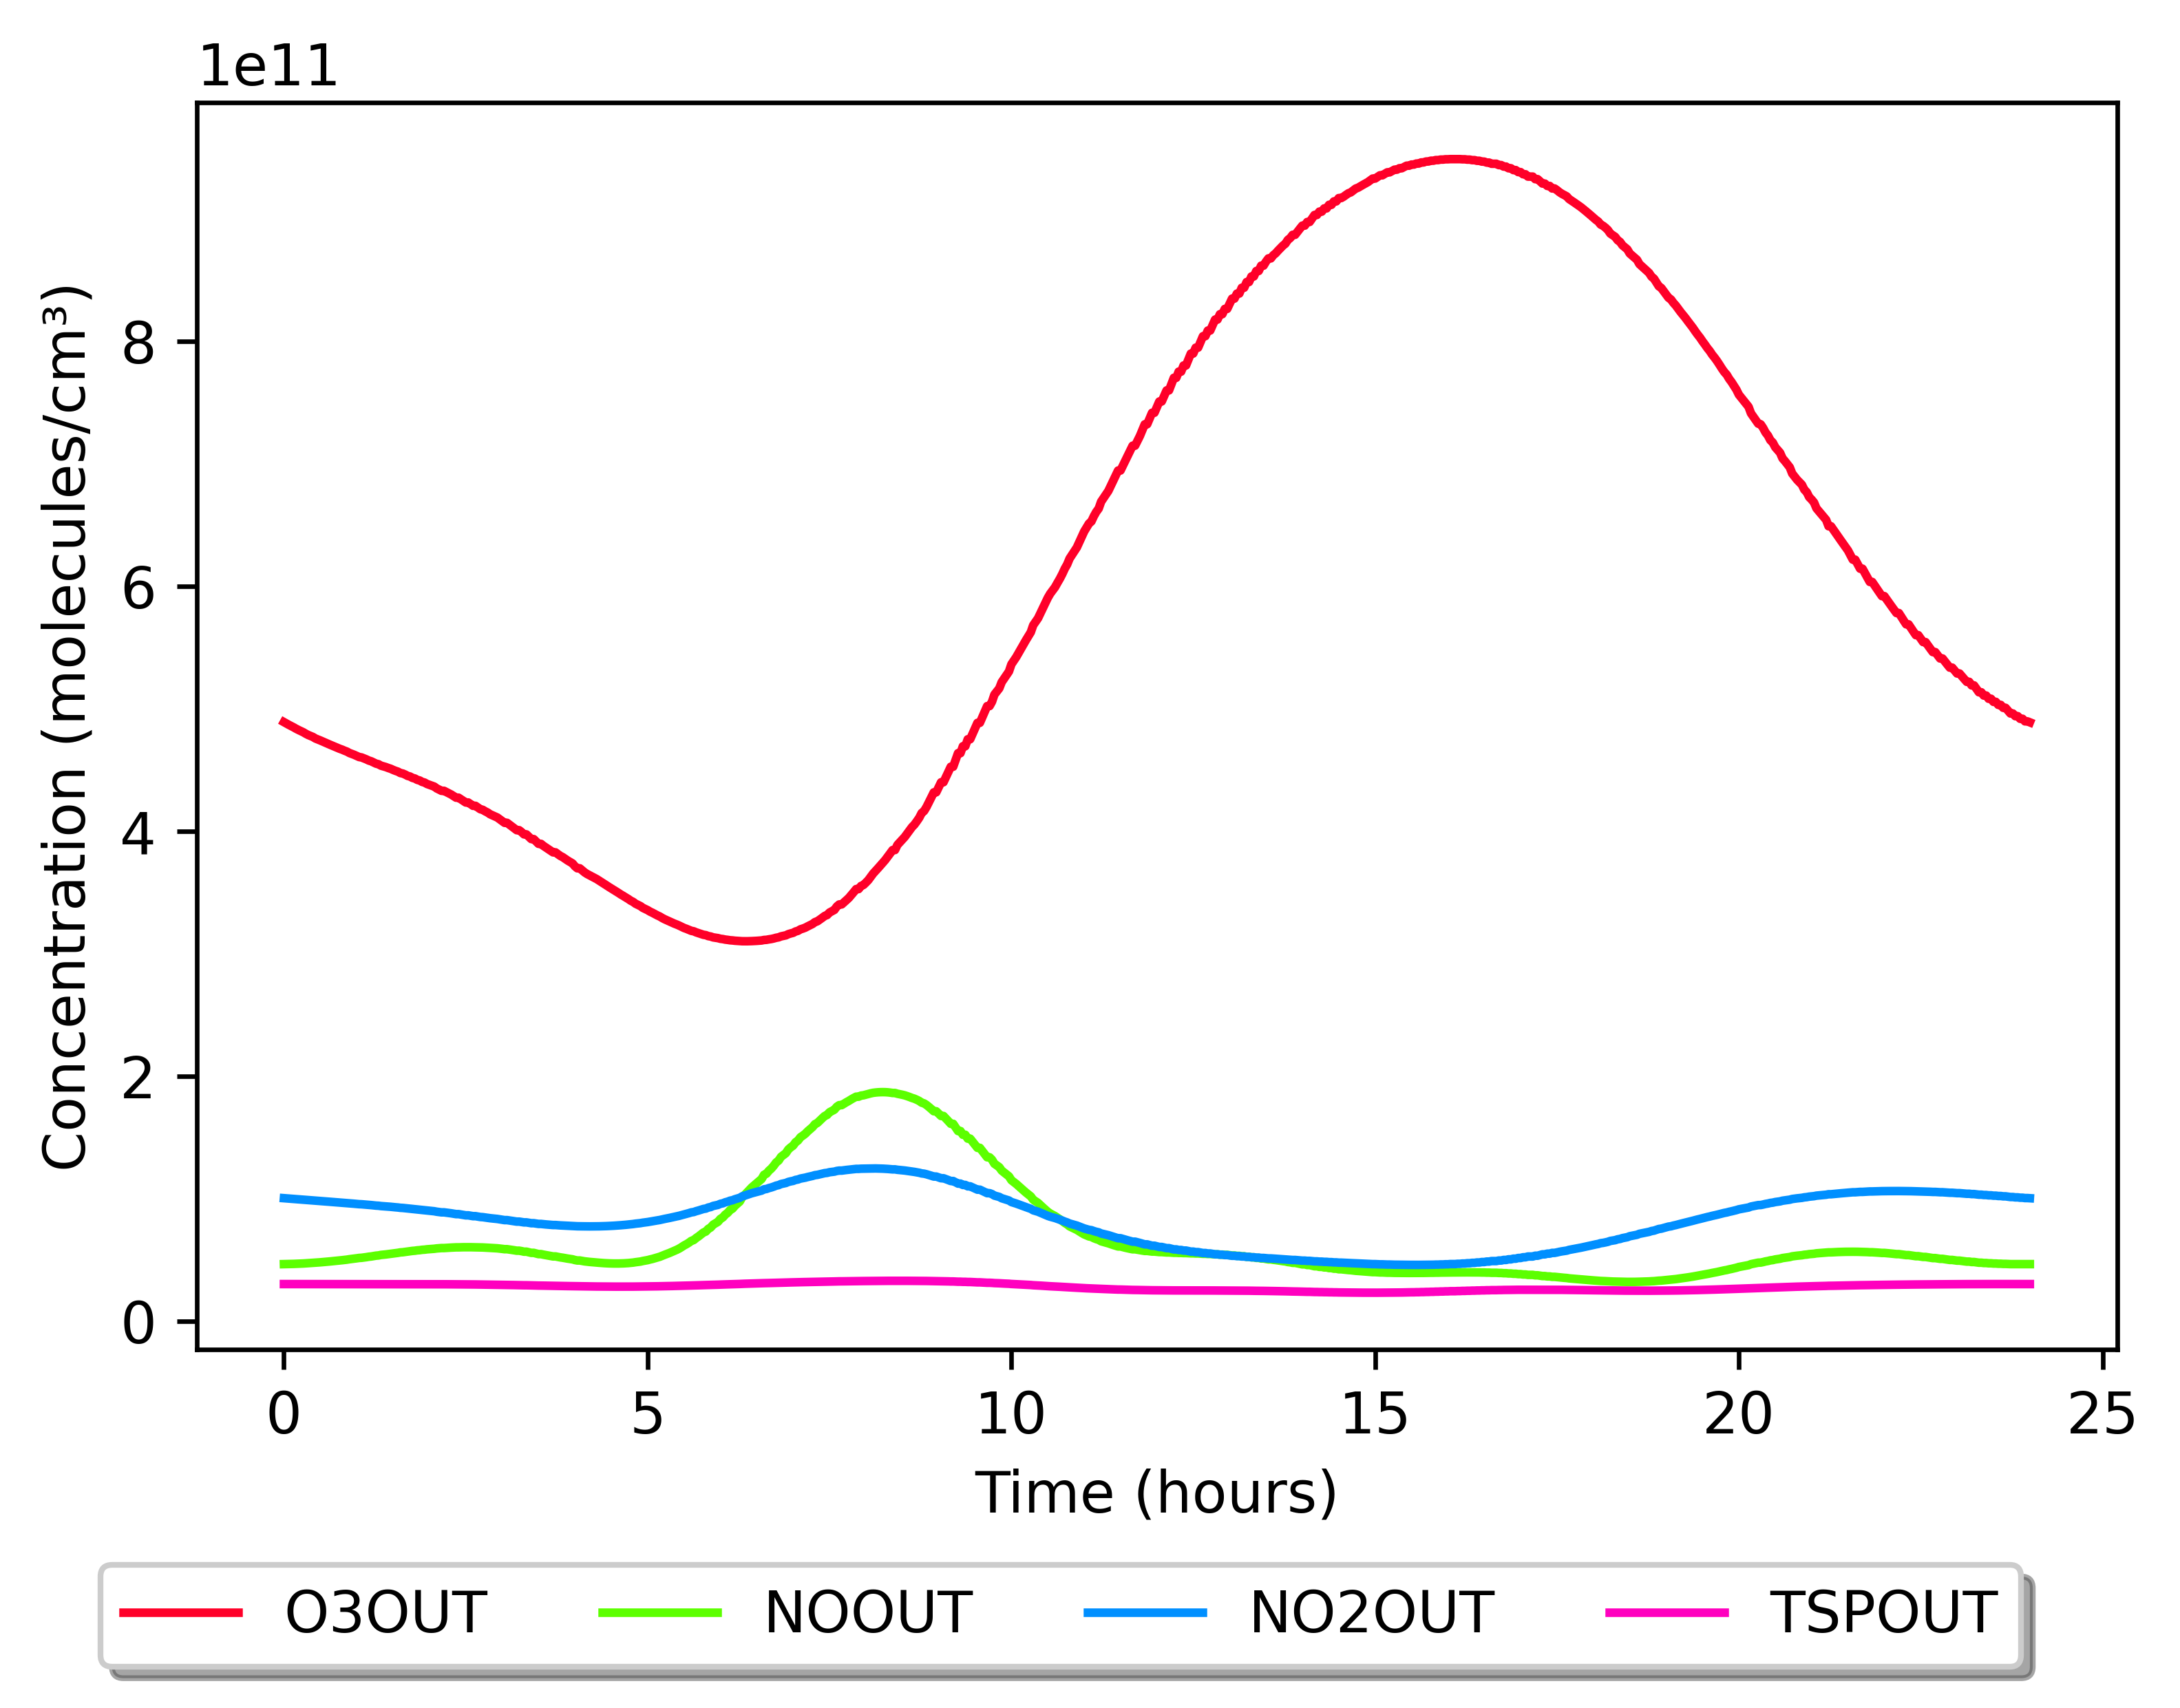
\includegraphics[width=\textwidth]{London_suburban.png}
    \caption{Outdoor average concentration fits for GB0586A, suburban London, Q3 2018.}
    \label{fig:Out_lon_sub}
\end{figure}
\begin{figure}[h!]
    \centering
    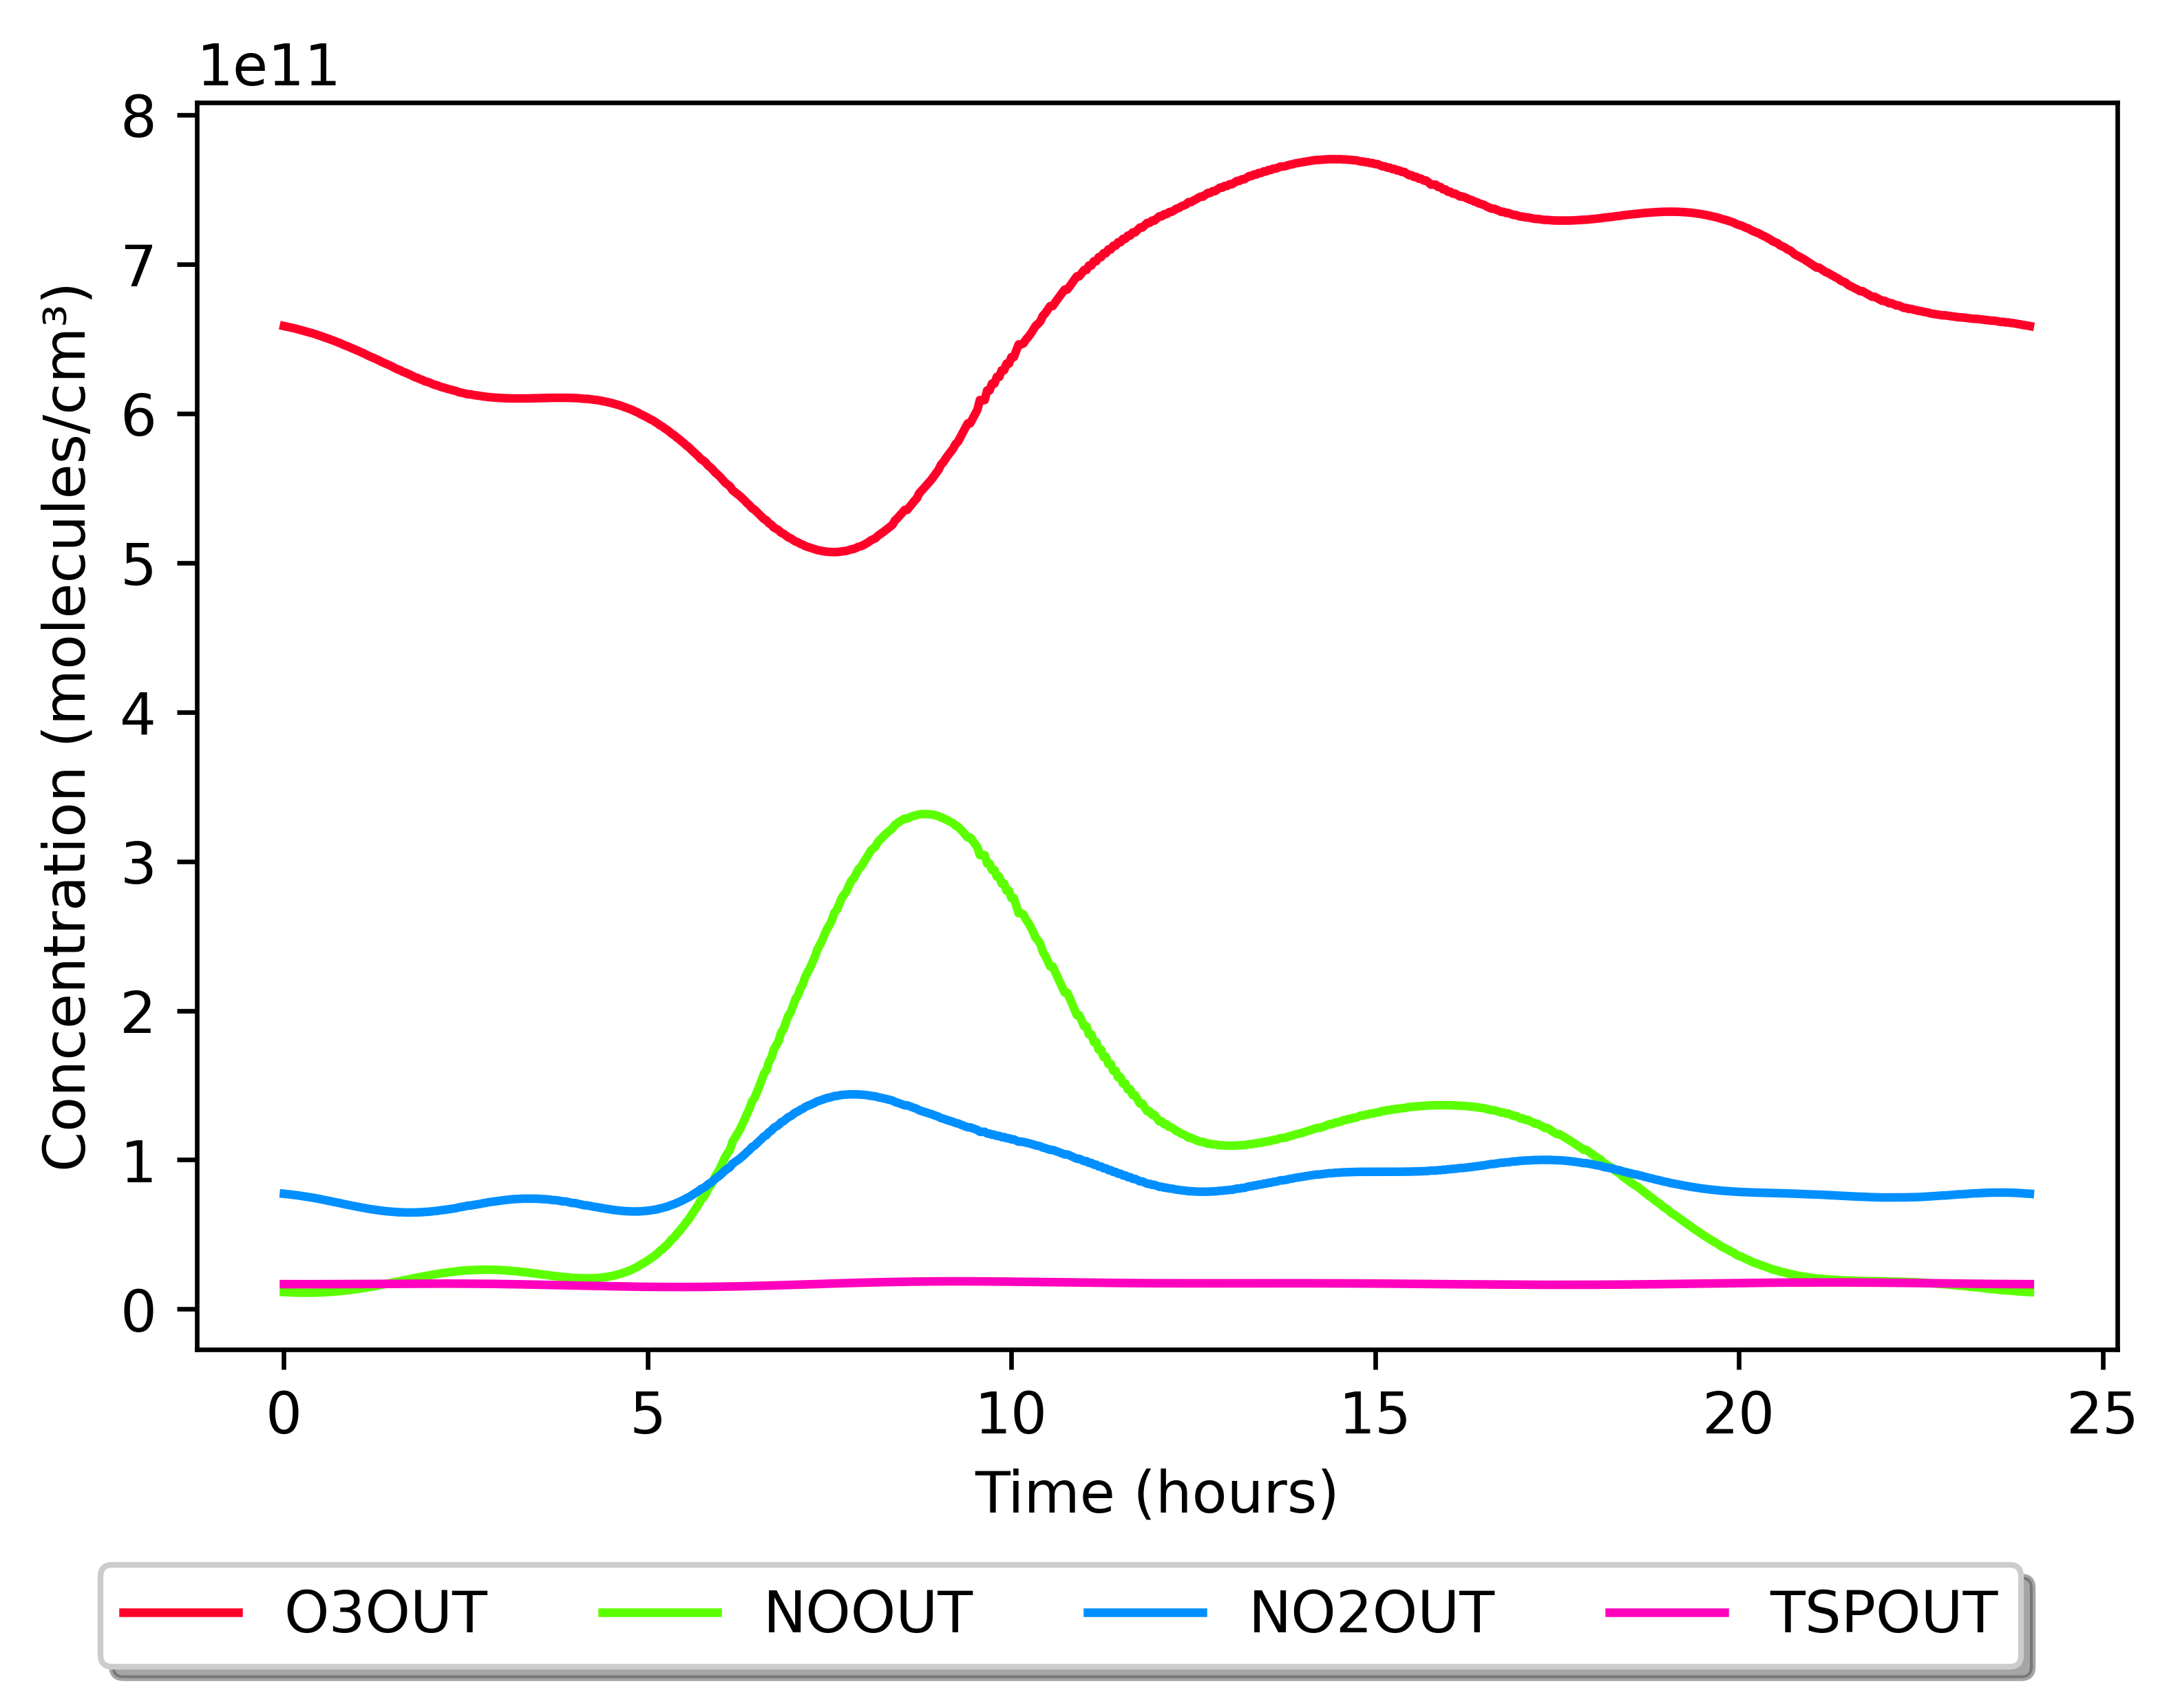
\includegraphics[width=\textwidth]{Bergen_urban.png}
    \caption{Outdoor average concentration fits for NO0120A, urban Bergen, Q3 2018.}
    \label{fig:Out_berg_urb}
\end{figure}
\begin{figure}[h!]
    \centering
    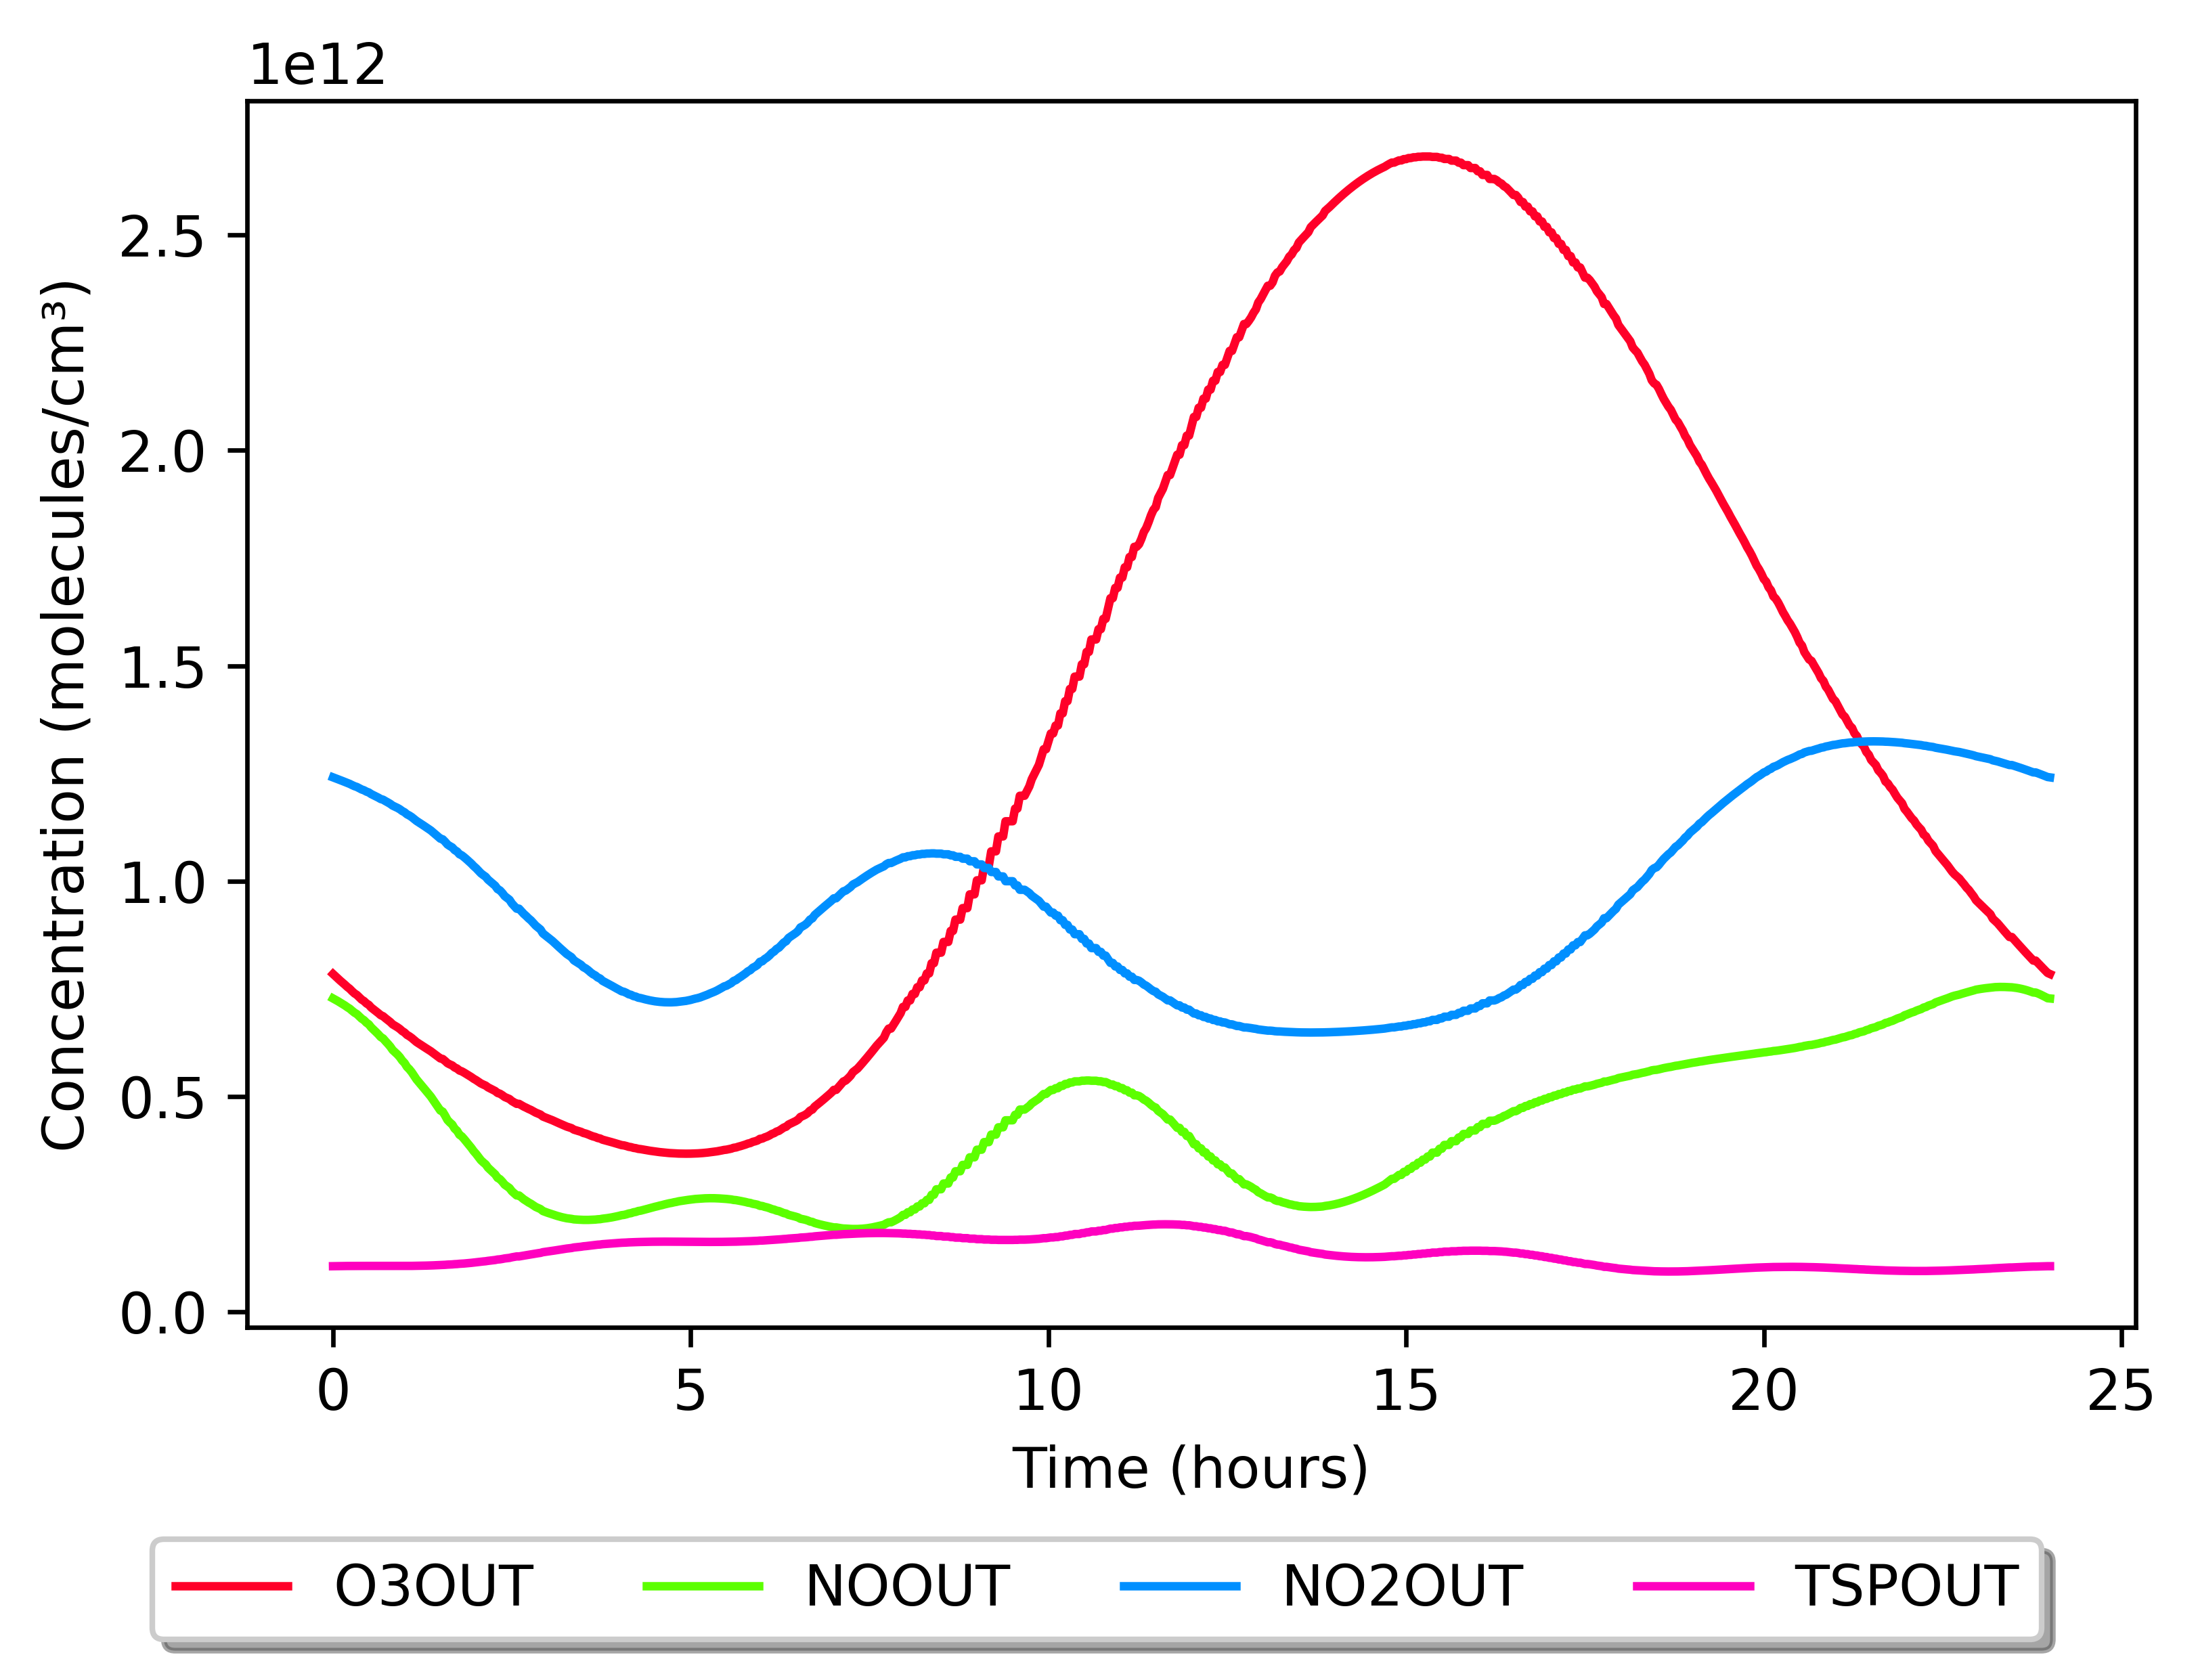
\includegraphics[width=\textwidth]{Milan_Aug2003.png}
    \caption{Outdoor concentration fits for a two week period in Milan in August 2003 \cite{Terry2014}.}
    \label{fig:Milan}
\end{figure}

\clearpage
\section{inchem\_extractor.py}\label{inchem_extractor.py}\index{inchem\_extractor.py}
inchem\_extractor.py will extract data from the out\_data.pickle files produced by INCHEM-Py and save the species concentrations, or other outputs that are specified, to a csv file. Multiple output files can be read at a time. Plots comparing results from any files input will be saved to an output folder to get quick and easy comparisons between model runs. 

This script is not part of INCHEM-Py but is additional to it to give greater accessibility to any users that are not comfortable with Python. It is intended to provide quick access to data, not as a tool for further analysis.

All elements that should be changed by the user are at the top of the file.

\marginlabel{out\_directories}
\begin{verbatim}
out_directories = ['directory1','directory2','directory3']
\end{verbatim}
A list of output folder names that inchem\_extractor will take output data from. These are created by INCHEM-Py when it is run in the format YYYYMMDD\_hhmmss\_custom and should be listed here. These names are not the full file path as this script expects to be one directory above these.

\marginlabel{species\_to\_extract}
\begin{verbatim}
species_to_extract = ['species1','species2','species3']
\end{verbatim}
A list of output variables to extract and plot. The script will differentiate between concentrations, reactivity, production rates and photolysis coefficients (if entered) and plot them on separate graphs with the correct axes labels. 

\marginlabel{start\_time and end\_time}
\begin{verbatim}
start_time = 0
end_time = 86400
\end{verbatim}
Time in seconds between which to plot the graphs. This does not change the data extracted to .csv files, the full simulation time range will always be extracted.

\marginlabel{scale}
\begin{verbatim}
scale = "hours"
\end{verbatim}
String to change the scale of the time axis on the plots. The options are "hours", "minutes", or "seconds". This does not change the data extracted to the .csv

\marginlabel{output\_folder}
\begin{verbatim}
output_folder = "folder_name"
\end{verbatim}
String name of output folder, that either exists already or is to be created, where the .csv files and plots are saved.

\marginlabel{log\_plot}
\begin{verbatim}
log_plot = True
\end{verbatim}
Can be True or False. True to set the y axis to a log scale, False to set the y axis to a linear scale.

\end{document}
